\documentclass[a4paper, 12pt]{article}

\def\languages{french, english}

%%%%%%%%%%%%%%%%%%% Libraries

%%%%%%%%%% Packages

\usepackage[
backend=biber,
style=numeric-comp,
sorting=none,
maxbibnames=99
]{biblatex}

\newgeometry{margin = 2.5cm}
\makeatletter
\begin{titlepage}
	\begin{minipage}[t][0.4125\textheight]{\textwidth}
		\begin{center}
		    \ifx\toptitle\undefined
    		    \ifx\logopath\undefined
    		    \else
    		    	\vfill
    			    \includegraphics[height=0.15\textheight]{\logopath}
    			\fi
    		\else
    		    \ifx\logopath\undefined
    		    \else
    			    \includegraphics[height=0.15\textheight]{\logopath}
    			\fi
    			\vfill
    			{\huge \textsc{\toptitle}}
			\fi
			\vfill
		\end{center}
	\end{minipage}
	\vfill
	\begin{minipage}{\textwidth}
		\hspace{0.5em}
		\begin{mdframed}[linewidth = 2pt, innertopmargin = 1em, innerbottommargin = 1em, leftline = false, rightline = false]
			\begin{center}
				{\huge \bfseries \@title}
			\end{center}
		\end{mdframed}
		\hspace{0.5em}
		\ifx\subtitle\undefined
		\else
		\begin{center}
			{\LARGE \subtitle}
		\end{center}
		\fi
	\end{minipage}
	\vfill
	\begin{minipage}[b][0.4125\textheight][t]{\textwidth}
			\vfill
			\ifx\rightauthor\undefined
			    \begin{center}
			        \ifx\authorhead\undefined
			        \else
		                {\large\it \authorhead\\[0.5em]}
		            \fi
			        {\large \@author}
			    \end{center}
			\else
			    \begin{minipage}[t]{0.5\textwidth}
			        \begin{flushleft}
			            \ifx\authorhead\undefined
			            \else
			                {\large\it \authorhead\\[0.5em]}
			            \fi
				        {\large \@author}
				    \end{flushleft}
				\end{minipage}
				\begin{minipage}[t]{0.5\textwidth}
				    \begin{flushright}
				        \ifx\rightauthorhead\undefined
			            \else
			                {\large\it \rightauthorhead\\[0.5em]}
			            \fi
				        {\large \rightauthor}
				    \end{flushright}
				\end{minipage}
			\fi
			\vfill
			\begin{center}
			    \ifx\context\undefined
			    \else
			        {\large \context \\[0.5em]}
			    \fi
			    {\large \@date}
			\end{center}
	\end{minipage}
\end{titlepage}
\makeatother
\restoregeometry
%%%%%%%%%% Packages

\usepackage{float}
\usepackage[skip=1em]{caption}

\usepackage{array}
\usepackage{multirow}
\usepackage{multicol}

%%%%%%%%%% Features

%%%%% Settings

\renewcommand{\arraystretch}{1.2}

%%%%% Commands

\newcommand\noskipcaption[1]{\caption{#1}\vspace{-1em}}
\newcommand\noskipcaptionstar[1]{\caption*{#1}\vspace{-1em}}

%%%%%%%%%% Packages

\usepackage{inconsolata}
\usepackage{listings}

%%%%%%%%%% Features

%%%%% Commands

\newcommand{\Nstyle}[1]{
    \lstdefinestyle{N#1}{
        style=#1,
        %%%%%
        numbers=left
    }
}

\newcommand{\tbFstyle}[1]{
    \lstdefinestyle{tbF#1}{
        style=#1,
        %%%%%
        frame=tb
    }
}

\newcommand{\Fstyle}[1]{
    \lstdefinestyle{F#1}{
        style=#1,
        %%%%%
        frame=single,
        framesep=0em,
        rulesep=0em,
        xleftmargin=0.75em,
        xrightmargin=0.75em,
        framexleftmargin=0.75em,
        framexrightmargin=0.75em,
        framextopmargin=0.5em,
        framexbottommargin=0.5em,
        %%%%%
        numbersep=1.25em
    }
}

\newcommand{\NtbFstyle}[1]{
    \tbFstyle{#1}
    \Nstyle{tbF#1}
}

\newcommand{\NFstyle}[1]{
    \Fstyle{#1}
    \lstdefinestyle{NF#1}{
        style=f#1,
        %%%%%
        xleftmargin=2.75em,
        framexleftmargin=2.75em,
        %%%%%
        numbers=left,
        numbersep=1em
    }
}

%%%%% Styles

\lstdefinestyle{default}{
    breaklines=true,
    breakatwhitespace=true,
    columns=fixed,
	extendedchars=true,
    upquote=true,
	tabsize=4,
    %%%%%
    framerule=0.66pt,
    captionpos=b,
	%%%%%
    basicstyle=\footnotesize\ttfamily,
    numberstyle=\footnotesize\ttfamily,
    showstringspaces=false
}
\Nstyle{default}
\NFstyle{default}
\NtbFstyle{default}

\lstdefinestyle{monokai}{
    style=Fdefault,
    %%%%%
    backgroundcolor=\color[HTML]{272822},
    framerule=0em,
    %%%%%
    basicstyle=\footnotesize\ttfamily\color[HTML]{f8f8f2},
    numberstyle=\footnotesize\ttfamily\color[HTML]{272822},
    commentstyle=\color[HTML]{75715e},
    keywordstyle=[1]{\color[HTML]{f92672}},
    keywordstyle=[2]{\color[HTML]{A6E22E}},
    keywordstyle=[3]{\color[HTML]{ae81ff}},
    stringstyle=\color[HTML]{e6db74},
    %%%%%
    % otherkeywords={!,.,+,-,*,/,=,<,>,^,|,\&,OR,AND}
}

\lstdefinestyle{Nmonokai}{
    style=monokai,
    %%%%%
    xleftmargin=2.75em,
    framexleftmargin=2.75em,
    %%%%%
    numbers=left,
    numberstyle=\footnotesize\ttfamily\color[HTML]{f8f8f2},
    numbersep=1em
}

\lstdefinestyle{c}{
    language=C,
    style=default,
    %%%%%
    commentstyle=\color[HTML]{228B22},
    keywordstyle=\color[HTML]{0000FF},
    stringstyle=\color[HTML]{A020F0},
    emphstyle=\color[HTML]{0000FF},
    %%%%%
    emph={}
}

\lstdefinestyle{cpp}{
    language=C++,
    style=default,
    %%%%%
    commentstyle=\color[HTML]{228B22},
    keywordstyle=\color[HTML]{0000FF},
    stringstyle=\color[HTML]{A020F0},
    emphstyle=\color[HTML]{0000FF},
    %%%%%
    emph={std}
}

\lstdefinestyle{matlab}{
    language=matlab,
    style=default,
    %%%%%
    basicstyle=\footnotesize\fontfamily{pcr}\selectfont,
    numberstyle=\footnotesize\fontfamily{pcr}\selectfont,
    commentstyle=\color[HTML]{228B22},
    keywordstyle=\color[HTML]{0000FF},
    stringstyle=\color[HTML]{A020F0},
    emphstyle=\color[HTML]{0000FF},
    %%%%%
    emph={clearvars}
}

\lstdefinestyle{python}{
    language=python,
    style=default,
    %%%%%
    commentstyle=\color[RGB]{221,0,0},
    keywordstyle=[1]{\color[RGB]{255,119,0}},
    keywordstyle=[2]{\color[RGB]{144,0,144}},
    stringstyle=\color[RGB]{0,170,0},
    emphstyle=\color[RGB]{255,119,0},
    %%%%%
    emph={}
}

\lstdefinestyle{java}{
    language=java,
    style=default,
    %%%%%
    commentstyle=\color[HTML]{228B22},
    keywordstyle=\color[HTML]{0000FF},
    stringstyle=\color[HTML]{A020F0},
    emphstyle=\color[HTML]{0000FF},
    %%%%%
    emph={}
}

%%%%%%%%%% Packages

\usepackage{amsmath}
\usepackage{amssymb}
\usepackage{bm}
\usepackage{esint}
\usepackage[makeroom]{cancel}

%%%%%%%%%% Features

%%%%% Macros

\newcommand{\rbk}[1]{\left(#1\right)}
\newcommand{\cbk}[1]{\left\{#1\right\}}
\newcommand{\sbk}[1]{\left[#1\right]}
\newcommand{\abs}[1]{\left|#1\right|}
\newcommand{\norm}[1]{\left\|#1\right\|}

\newcommand{\fact}[1]{#1!}
\newcommand{\e}[1]{\mathbf{e}_{#1}}
\newcommand{\deriv}{\mathrm{d}}
\DeclareMathOperator{\tr}{tr}

\def\Rl{\mathbb{R}}
\def\Cx{\mathbb{C}}
\def\Na{\mathbb{N}}
\def\Zi{\mathbb{Z}}

%%%%%%%%%% Packages

\usepackage{amsthm}
\usepackage{thmtools}

%%%%%%%%%% Features

%%%%% Settings

\makeatletter
\define@key{thmdef}{mdthm}[{}]{
	\thmt@trytwice{\def\thmt@theoremdefiner{\mdtheorem[#1]}}{}}
\makeatother

\begingroup
\makeatletter
\@for\theoremstyle:=plain,definition,remark\do{
	\expandafter\g@addto@macro\csname th@\theoremstyle\endcsname{
		\addtolength\thm@preskip\parskip
	}
}
\endgroup

\renewcommand{\qedsymbol}{$\blacksquare$}

% language

\ifx\lgthm\undefined
	\def\lgthm{Theorem}
	\def\lgprf{Proof}
	\def\lglem{Lemma}
	\def\lgprop{Proposition}
	\def\lgdefn{Definition}
	\def\lghyp{Hypothesis}
	\def\lgmeth{Method}
	\def\lgquest{Question}
	\def\lgansw{Answer}
	\def\lgexpl{Example}
	\def\lgrmk{Remark}
	\def\lgnote{Note}
	\def\lgtip{Tip}
\fi

%%%%% Commands

\newcommand\qedadd{\pushQED{\qed}\popQED}

%%%%% Environments

\theoremstyle{plain}
\newtheorem{thm}{\lgthm}
\newtheorem{lem}[thm]{\lglem}
\newtheorem{prop}[thm]{\lgprop}

\theoremstyle{definition}
\newtheorem{defn}{\lgdefn}
\newtheorem{hyp}{\lghyp}
\newtheorem{meth}{\lgmeth}
\newtheorem{quest}{\lgquest}

\theoremstyle{remark}
\newtheorem{answ}{\lgansw}[quest]
\newtheorem{expl}{\lgexpl}
\newtheorem*{rmk}{\lgrmk}
\newtheorem*{note}{\lgnote}
\newtheorem*{tip}{\lgtip}

% framed

\mdfdefinestyle{thicc}{
	nobreak=true,
	skipabove=\topskip,
	skipbelow=\topskip,
	innerleftmargin=0.5em,
	innerrightmargin=0.5em,
	innerbottommargin=0.5em,
	innertopmargin=0.5em,
	linewidth=0.25em,
	roundcorner=0.15em,
	linecolor=black!10,
	frametitlebackgroundcolor=black!10,
	theoremseparator={.}
}

\declaretheorem[mdthm={style=thicc, linecolor=red!20, frametitlebackgroundcolor=red!20}, sibling=thm, name=\lgthm]{framedthm}
\declaretheorem[mdthm={style=thicc, linecolor=red!20, frametitlebackgroundcolor=red!20}, sibling=thm, name=\lglem]{framedlem}
\declaretheorem[mdthm={style=thicc, linecolor=blue!20, frametitlebackgroundcolor=blue!20}, sibling=thm, name=\lgprop]{framedprop}
\declaretheorem[mdthm={style=thicc, nobreak=false}, parent=thm, name=\lgprf]{framedprf}

\declaretheorem[mdthm={style=thicc, linecolor=black!20!green!20, frametitlebackgroundcolor=black!20!green!20}, sibling=defn, name=\lgdefn]{frameddefn}
\declaretheorem[mdthm={style=thicc, linecolor=blue!20, frametitlebackgroundcolor=blue!20}, sibling=hyp, name=\lghyp]{framedhyp}
\declaretheorem[mdthm={style=thicc}, name=\lgmeth]{framedmeth}
\declaretheorem[mdthm={style=thicc, linecolor=orange!20, frametitlebackgroundcolor=orange!20}, sibling=quest, name=\lgquest]{framedquest}

\declaretheorem[mdthm={style=thicc, nobreak=false}, sibling=answ, name=\lgansw]{framedansw}
\declaretheorem[mdthm={style=thicc, nobreak=false}, sibling=expl, name=\lgexpl]{framedexpl}

%%%%%%%%%% Packages

\usepackage{siunitx}

%%%%%%%%%% Features

%%%%% Settings

\ifx\decimalsign\undefined
\else
    \sisetup{output-decimal-marker = \decimalsign}
\fi


%%%%%%%%%%%%%%%%%%% Titlepage

\def\logopath{resources/pdf/logo-uliege.pdf}
\def\toptitle{University of Liège}
\title{Study of an active mass damper}
\def\subtitle{Linear control systems}
%\def\authorhead{Author}
\author{
    Bastien \textsc{Hoffmann} (20161283)\\
    Maxime \textsc{Meurisse} (20161278)\\
    Valentin \textsc{Vermeylen} (20162864)\\
}
%\def\rightauthorhead{}
%\def\rightauthor{}
\def\context{Master in Civil Engineering}
\date{Academic year 2019-2020}

%%%%%%%%%%%%%%%%%%% Options

\fancyhead[R]{}
\addbibresource{references.bib}
\defbibheading{bibliography}[\refname]{}

%%%%%%%%%%%%%%%%%%% Document

\begin{document}
    % ----- Titlepage ----- %
    \newgeometry{margin = 2.5cm}
\makeatletter
\begin{titlepage}
	\begin{minipage}[t][0.4125\textheight]{\textwidth}
		\begin{center}
		    \ifx\toptitle\undefined
    		    \ifx\logopath\undefined
    		    \else
    		    	\vfill
    			    \includegraphics[height=0.15\textheight]{\logopath}
    			\fi
    		\else
    		    \ifx\logopath\undefined
    		    \else
    			    \includegraphics[height=0.15\textheight]{\logopath}
    			\fi
    			\vfill
    			{\huge \textsc{\toptitle}}
			\fi
			\vfill
		\end{center}
	\end{minipage}
	\vfill
	\begin{minipage}{\textwidth}
		\hspace{0.5em}
		\begin{mdframed}[linewidth = 2pt, innertopmargin = 1em, innerbottommargin = 1em, leftline = false, rightline = false]
			\begin{center}
				{\huge \bfseries \@title}
			\end{center}
		\end{mdframed}
		\hspace{0.5em}
		\ifx\subtitle\undefined
		\else
		\begin{center}
			{\LARGE \subtitle}
		\end{center}
		\fi
	\end{minipage}
	\vfill
	\begin{minipage}[b][0.4125\textheight][t]{\textwidth}
			\vfill
			\ifx\rightauthor\undefined
			    \begin{center}
			        \ifx\authorhead\undefined
			        \else
		                {\large\it \authorhead\\[0.5em]}
		            \fi
			        {\large \@author}
			    \end{center}
			\else
			    \begin{minipage}[t]{0.5\textwidth}
			        \begin{flushleft}
			            \ifx\authorhead\undefined
			            \else
			                {\large\it \authorhead\\[0.5em]}
			            \fi
				        {\large \@author}
				    \end{flushleft}
				\end{minipage}
				\begin{minipage}[t]{0.5\textwidth}
				    \begin{flushright}
				        \ifx\rightauthorhead\undefined
			            \else
			                {\large\it \rightauthorhead\\[0.5em]}
			            \fi
				        {\large \rightauthor}
				    \end{flushright}
				\end{minipage}
			\fi
			\vfill
			\begin{center}
			    \ifx\context\undefined
			    \else
			        {\large \context \\[0.5em]}
			    \fi
			    {\large \@date}
			\end{center}
	\end{minipage}
\end{titlepage}
\makeatother
\restoregeometry
    
    % ----- Table of contents ----- %
    \romantableofcontents
    
    % ----- Control problem ----- %
    \section{Control problem}

% Choice of the topic
\subsection{Choice of the topic}
The chosen topic is : {\bf Active mass damper}.

% Context
\subsection{Context}
The current engineering prowesses allow us to construct buildings higher and higher. These constructions are subject to various disturbances (mainly wind, but also earthquakes) that make them oscillate. They turn into giant pendulum and swing from left to right, sometimes moving several meters at the top !\cite{YouTube_minutephysics}\par
To reduce these oscillations, we use a passive system, called {\it tuned mass damper}, which consists of concealing a tuned and harmonic oscillator at the top of the tower. It is coupled to its movement and oscillates in phase opposition to recover the kinetic energy of the tower and thus reduces the oscillations.\cite{Wikipedia_amortisseur_tmd}\par
An active version of this system exists : the {\it active mass damper}. It consists of the same principle as the tuned mass damper but it is equipped with sensors and actuators to measure the oscillations of its environment and, via an algorithm, generate a movement for the mass that reduce, or totally remove, these oscillations.\cite{sciencedirect_amd}\par
Our study field focuses on the active mass damper systems used to reduce the oscillations caused by the {\bf wind} on {\bf tall} buildings.

% Control problem diagram
\subsection{Control problem diagram}
The diagram of our control problem is shown in figure \ref{fig:diagram}.
\begin{figure}[!ht]
    \centering
    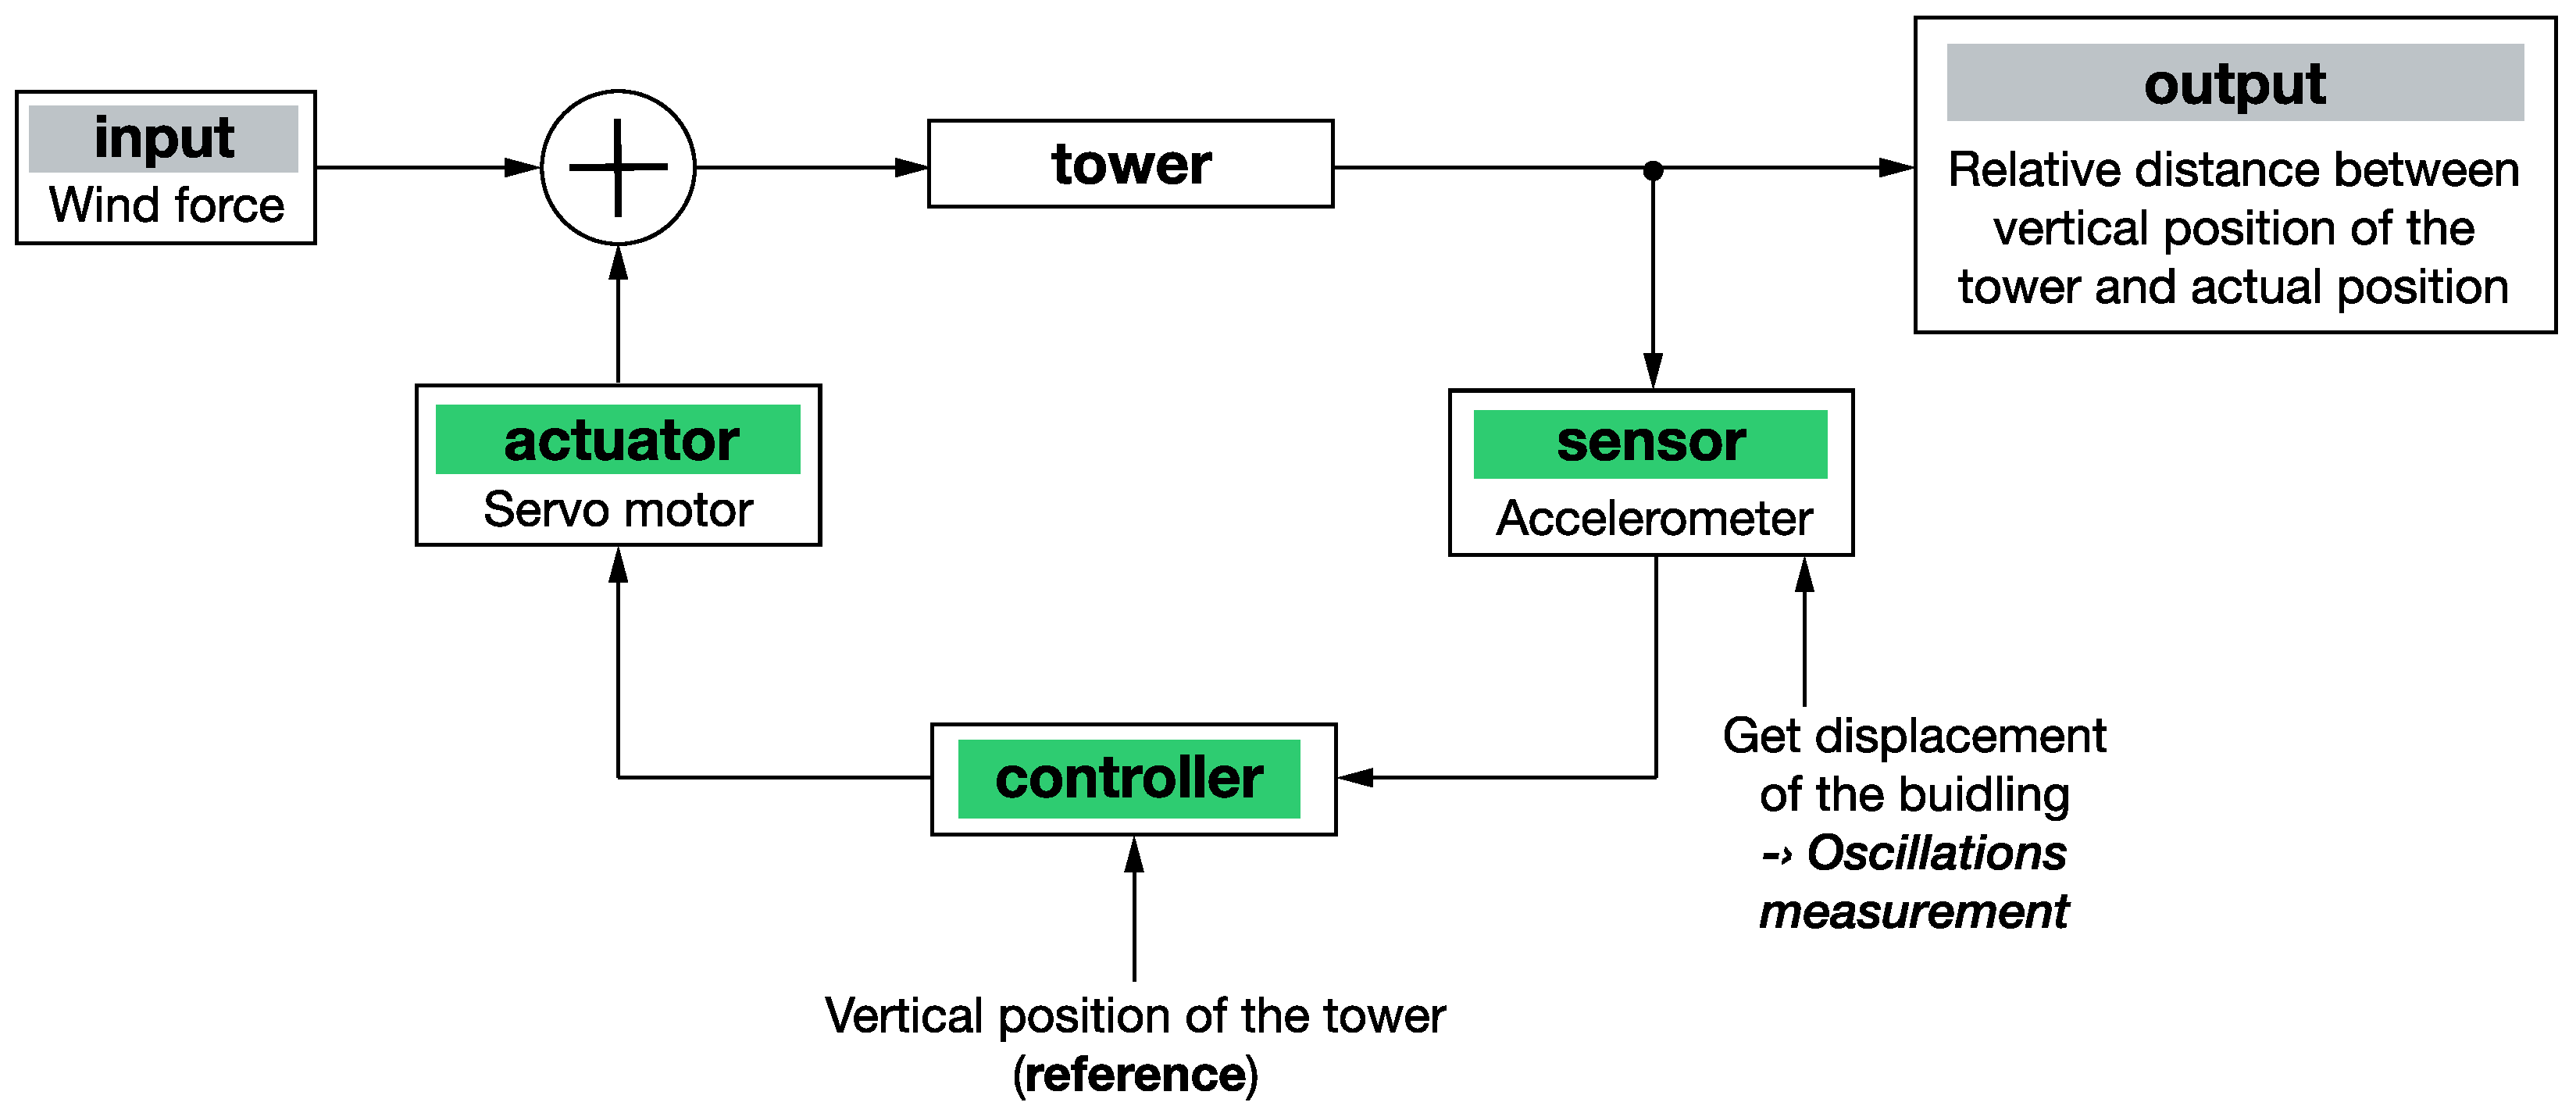
\includegraphics[width=1\textwidth]{resources/pdf/control-problem-diagram.pdf}
    \caption{Control problem diagram of the active mass damper for tall buildings}
    \label{fig:diagram}
\end{figure}

% Control problem description
\subsection{Control problem description}
\begin{itemize}
    \item {\bf Utility of the controller} : the controller (the algorithm) allows the system (the tower) to be active, {\it i.e.} to measure the oscillations to which it is subjected and to cancel it. Thanks to a servo-motor connected to the controller, the mass can move and reduce, or even eliminate totally, the oscillations.
    \item {\bf System to be controlled} : the tower (and the position of the tower is the signal)
    \item {\bf Inputs of the system} : wind force acting on the tower (uncontrollable) and force acting on the mass damper (controllable).
    \item {\bf Outputs of the system} : the relative distance between the vertical position and the displacement of the tower.
    \item {\bf Reference} : the vertical position of the tower.
    \item {\bf Actuators} : servo-motor to move the mass that reduces the oscillations.
    \item {\bf Constraints and limitations} : to simplify our system, we consider a tower \SI{200}{\meter} high, perfectly vertical when it undergoes no disturbance. The only disturbance on this tower is the strength of the wind. The wind, ranging from a few tens of \SI{}{\kilo\meter/\hour} to a hundred \SI{}{\kilo\meter/\hour}, can swing the tower from a few centimetres to several meters.
\end{itemize}

% Open loop system diagram
\subsection{Open loop system diagram}
The detailed schematic of the open loop studied system is shown in figure \ref{fig:detailed_schematic}.
\begin{figure}[H]
    \centering
    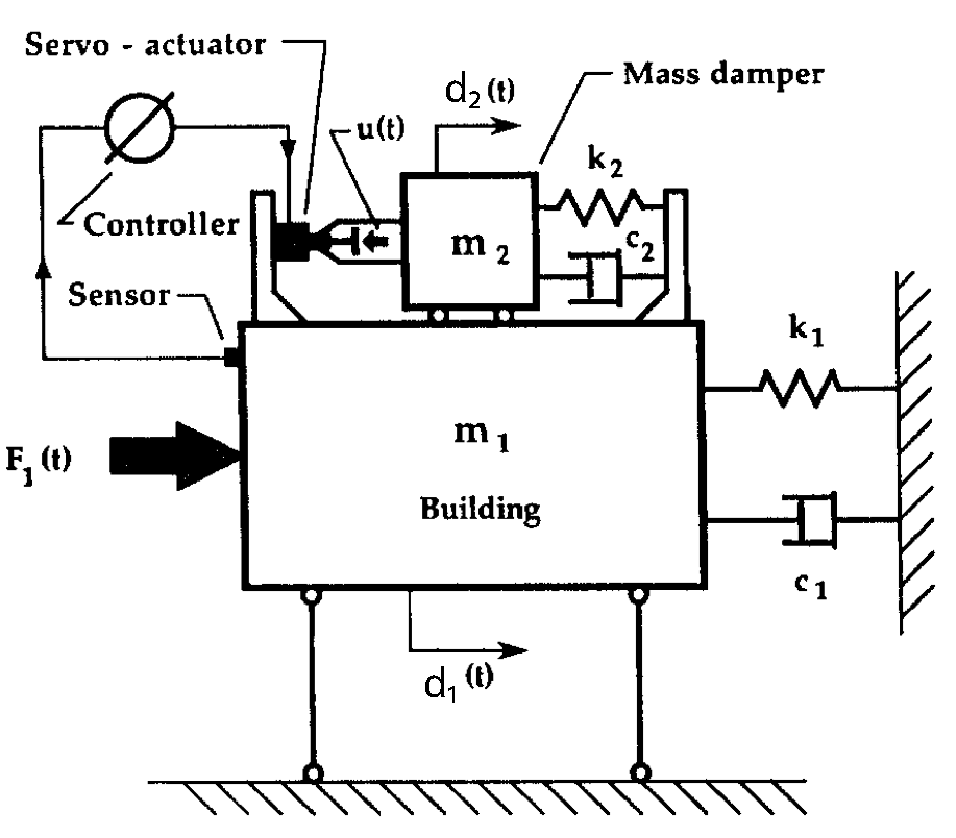
\includegraphics[width=0.7\textwidth]{resources/pdf/open-loop-diagram.pdf}
    \caption{Detailed schematic of the open loop studied system \cite{sciencedirect_amd}}
    \label{fig:detailed_schematic}
\end{figure}
The building is represented by the mass $m_1$ and its oscillation motion is simulated by the spring $k_1$ and the damper $c_1$.\par
The mass damper is represented by the mass $m_2$ and its movement is simulated by the spring $k_2$ and the damper $c_2$.\par
The force $F_1(t)$ represents the wind force (uncontrollable) on the building.\par
The force $u(t)$ represents the force applied on the mass damper by the controller (controllable).\par
We are studying, at first, our system without a control mechanism. Our controllable input $u(t)$ will therefore be \num{0} for all our simulations in this section.

    
    % ----- State-space representation ----- %
    \section{State-space representation}\label{state-space}

% Open loop model description
\subsection{Open loop model description}
Input vector $U$ and state vector $X$ are given by :
$$
U = \begin{pmatrix}
    F_1 \\
    u
\end{pmatrix}
\hspace{3cm}
X = \begin{pmatrix}
    d_1 \\
    \dot d_1 \\
    d_2 \\ 
    \dot d_2 \\
\end{pmatrix}
$$

\subsubsection{Inputs}
\begin{itemize}
    \item $F_1(t)$, the force of the wind (uncontrollable), between \num{500} and \SI{1500}{\kilo\newton} (which corresponds to a wind speed of \num{10} to \SI{15}{\meter\per\second} on our building).
    \item $u(t)$, the force applied on the mass damper (controllable), in the order of \SI{500}{\kilo\newton}.
\end{itemize}
The sensor considered is a measurement of the horizontal position of the top of the building relatively to the vertical position $d_1 = 0$.\par
The actuator provides a force on the mass of the dampener ($u(t)$), sets it in motion.

\subsubsection{Outputs}
$y = d_1(t)$ the relative position of the building with respect to the vertical position.

\subsubsection{States}
\begin{itemize}
    \item $x_1 = d_1$, as described above, ranging from a few millimeters to a few centimeters.
    \item $x_2 = \dot d_1$, the speed of the building, ranging from about \num{0} to \SI{5}{\meter\per\second}.
    \item $x_3 = d_2$, the relative displacement of the mass damper, ranging from about \num{0} to \SI{5}{\meter}.
    \item $x_4 = \dot d_2$, the speed of the mass damper, ranging from about \num{0} to \SI{10}{\meter\per\second}.
\end{itemize}

\subsubsection{Output law}
The output is one of the states : $y = x_1$.

\subsubsection{Update law}
The update law is given by \cite{YANG201718} :
$$
\begin{cases}
    m_{1}\ddot{d}_{1} + c_{1}\dot{d}_{1} + k_{1}d_{1} = c_{2}\dot{z} + k_{2}z + F_{1}(t) - u(t)\\
    m_{2}\ddot{z} + c_{2}\dot{z} + k_{2}z = -m_{2}\ddot{d}_{1} + u(t)
\end{cases}
$$
with $z = d_2 - d_1$.

% State-space model
\subsection{State-space model}
The system is \textbf{linear}. The ABCD matrices can be easily derived.
$$
A = \begin{pmatrix}
    0 & 1 & 0 & 0 \\
    \frac{-k_1-k_2}{m_1} & \frac{-c_2-c_1}{m_1} & \frac{k_2}{m_1} & \frac{c_2}{m_1} \\
    0 & 0 & 0 & 1 \\ 
    \frac{k_2}{m_2} & \frac{c_2}{m_2} & \frac{-k_2}{m_2} & \frac{-c_2}{m_2}\\
\end{pmatrix}
\quad
B = \begin{pmatrix}
    0 & 0\\
    \frac{1}{m_1} & -\frac{1}{m_1}\\
    0 & 0\\
    0 & \frac{1}{m_2}\\
\end{pmatrix}
$$
$$
C = \begin{pmatrix}
    1 & 0 & 0 & 0\\
\end{pmatrix}
\quad
D = \begin{pmatrix}
    0 & 0\\
\end{pmatrix}
$$

% Constraints, limitations and numerical choice of parameter values
\subsection{Constraints, limitations and numerical choice of parameter values}
To model and study the system, a series of constraints have to be defined, as well as assumptions and limitations.

\subsubsection{Basic system constraints}
The basic modeling constraints of our system are presented in table \ref{tab:constraints_assumptions_limitations}.\par
\begin{table}[H]
    \centering
    \begin{tabular}{|l|c|}
        \hline
        \multirow{2}{*}{{\bf Building}} & height of \SI{200}{\meter}, width of \SI{30}{\meter}\\ & movement along a single axis (horizontal)\\\hline
        {\bf Mass} & no friction between $m_1$ and $m_2$\\ \hline
    \end{tabular}
    \caption{Basic system constraints}
    \label{tab:constraints_assumptions_limitations}
\end{table}

\subsubsection{Constraints on signals}
The constraints on the different signals of our system\footnote{Given by our common sense and computations for the uncontrollable input. The maximum value of the controllable input corresponds to an acceleration of $1.6g$.} are presented in table \ref{tab:constraints_signals}.
\begin{table}[H]
    \centering
    \begin{tabular}{|l|m{8cm}|}
        \hline
        {\bf Reference} & a few millimeters or even a few centimeters at most (we expect it to remain 0mm)\\ \hline
        {\bf Controllable input} & in the order of \SI{500}{\kilo\newton}\\ \hline
        {\bf Uncontrollable input} & between \num{500} and \SI{1500}{\kilo\newton}\\ \hline
        {\bf Output} & from a few millimeters to a few centimeters (we don't want it to exceed 1m)\\ \hline
    \end{tabular}
    \caption{Constraints on signals}
    \label{tab:constraints_signals}
\end{table}

\subsubsection{Numerical values for simulations}
\label{sec:numerical_values}
To simulate the system (without control mechanism), a series of numerical values, presented in table \ref{tab:numerical_values}\footnote{We would like to thank Professor Denoël for discussing these values with us.} were chosen.
\begin{table}[H]
    \centering
    \begin{tabular}{|l|c|c|}
        \hline
        {\bf Mass} & $m_1 = \SI{1e7}{\kilogram}$ & $m_2 = \SI{3e4}{\kilogram}$\\ \hline
        {\bf Spring} & $k_1 \approx \SI{4e8}{\newton/\meter}$ & $k_2 = \SI{e5}{\newton/\meter}$\\ \hline
        {\bf Damper} & $c_1 \approx \SI{1.3e6}{\newton\second/\meter}$ & $c_2 = \SI{e4}{\newton\second/\meter}$\\ \hline
        {\bf Wind} & \multicolumn{2}{c|}{$F_{max} = \SI{810000}{\newton}$}\\ \hline
    \end{tabular}
    \caption{Numerical values of the system}
    \label{tab:numerical_values}
\end{table}
The stiffness and viscosity values for the building were obtained using the formulas :
\begin{align*}
    k_1 &= (2\pi f)^2m_1\\
    c_1 &= m_1\pi f0.04
\end{align*}
where $f = \SI{1}{\hertz}$ is the natural frequency associated with the mass of the building.\par
The maximum wind force, on the other hand, was approximated by
\begin{equation*}
    F_{max} = \frac{1}{2}\rho v^2A
\end{equation*}
with
\begin{itemize}
    \item $\rho \approx \SI{1.2}{\kilogram/\meter\cubed}$, the air density;
    \item $v = \SI{15}{\meter/\second}$, the wind speed;
    \item $A = 200\times 30 = \SI{6000}{\meter\squared}$, the area of one side of the building.
\end{itemize}
\paragraph{Scenarios considered}
For the uncontrollable input (wind), multiple scenarios were considered :
\begin{align*}
    F_1 &= F_{max}\quad\forall t & \text{Constant wind force}\\
    F_1(t) &= F_{max}\sin(2\pi t) & \text{Sinusoidal wind force}\\
    F_1(t) &= F_{max}\texttt{rand()} & \text{Random wind force}\\
\end{align*}
A constant force over time is not very realistic for wind but allows us to observe the behaviour of our system in the face of a very simple entry.\par
A sinusoidal force is also not very realistic but could correspond to multiple wind gusts on either side of the building.\par
A random wind is a rather realistic scenario that can model multiple wind gusts of varying intensity on either side of the building.

% Stability and eigenvalues
\subsection{Stability and eigenvalues}
\label{sec:eigenvalues}
To study the stability of the system, we computed the eigenvalues of the dynamic matrix $A$ thanks to Matlab function (\texttt{eig}) :
\begin{align*}
    \lambda_1 &= \num{-0.0634 + 6.2837i}\\
    \lambda_2 &= \num{-0.0634 - 6.2837i}\\
    \lambda_3 &= \num{-0.1666 + 1.8179i}\\
    \lambda_4 &= \num{-0.1666 - 1.8179i}
\end{align*}
The system is stable if the real parts of the eigenvalue are all negative. In this case, the system is thus stable.\par
We notice that $\lambda_1$ and $\lambda_2$, being closer to the imaginary axis than $\lambda_3$ and $\lambda_4$, are two dominant eigenvalues. They therefore govern the dynamics of the system.\par
We also note that $\lambda_3$ and $\lambda_4$ are also very close to the imaginary axis. So our system is very responsive.

% Open loop system simulations
\subsection{Open loop system simulations}
We simulated during 30 seconds, in open loop, the different scenarios presented in section \ref{sec:numerical_values}. We also varied the initial conditions. Since we have not yet implemented a control mechanism, the controllable input of the system is at 0 for all simulations. It can be noted that the open-loop system is already \og{}controlled\fg{} by a tuned mass damper.

\subsubsection{Initial conditions}
For this simulation, we changed the initial conditions of our system without applying wind force. We have defined that the initial displacement of our building (state $x_1$) is \SI{0.003}{\meter}.
\begin{figure}[H]
    \centering
    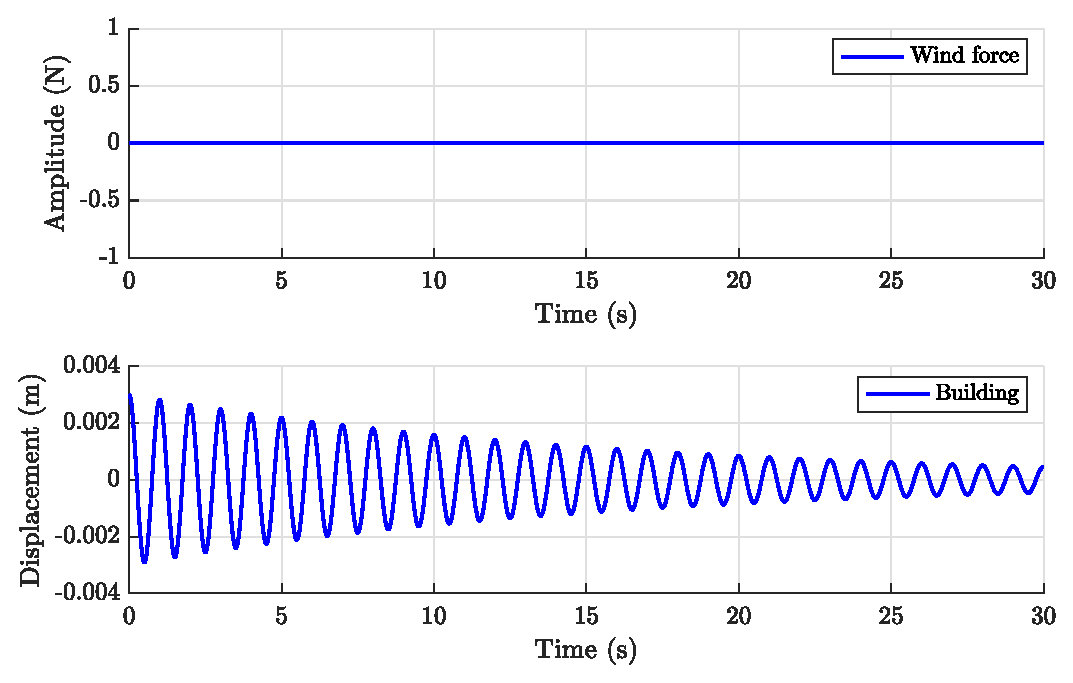
\includegraphics[width=\textwidth]{resources/eps/2_initial-conditions.eps}
    \caption{Open loop simulation during \SI{30}{\second} with initial conditions ($x_1=\SI{0.003}{\meter}$)}
\end{figure}
We can see that our system is very reactive: the building oscillates quite quickly. It also quickly regains a position oscillating close to its reference position.

\subsubsection{Constant wind force}
For this simulation, we applied a constant wind with zero initial conditions.
\begin{figure}[H]
    \centering
    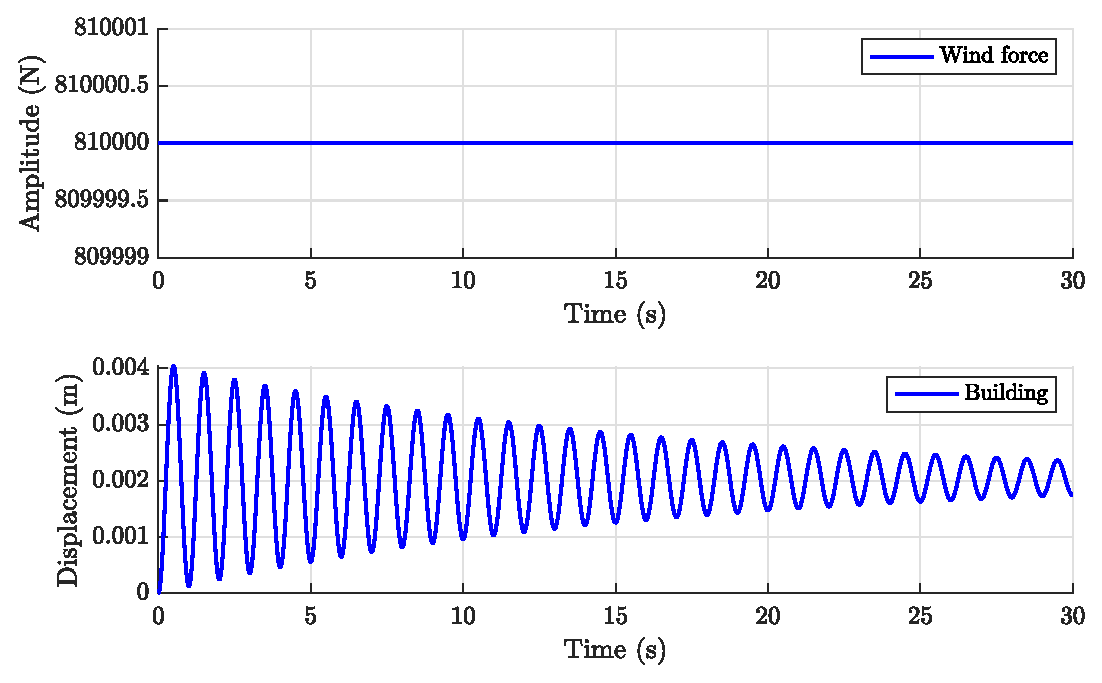
\includegraphics[width=\textwidth]{resources/eps/2_constant-wind.eps}
    \caption{Open loop simulation during \SI{30}{\second} for a constant wind force ($x_1=\SI{0}{\meter}$)}
\end{figure}
In this case, we can see that the building also oscillates very quickly. The displacement decreases quickly over time to finally oscillate around a position slightly different from its reference position.

\subsubsection{Sinusoidal wind force}
For this simulation, we applied a sinusoidal wind with zero initial conditions.
\begin{figure}[H]
    \centering
    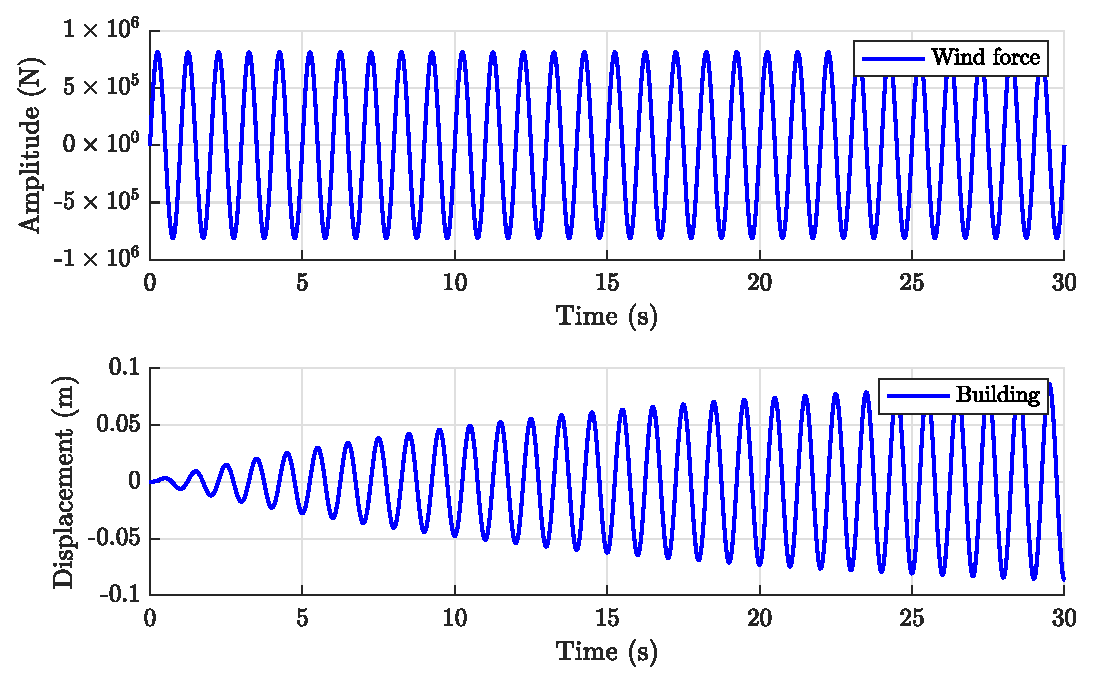
\includegraphics[width=\textwidth]{resources/eps/2_sinusoidal-wind.eps}
    \caption{Open loop simulation during \SI{30}{\second} for a sinusoidal wind force ($x_1=\SI{0}{\meter}$)}
\end{figure}
We can see that the building's oscillations gradually increase, but quite rapidly, over time. A longer simulation has shown that these oscillations stabilize at a maximum value of \SI{0.1}{\meter} after about 30 seconds.

\subsubsection{Random wind force}
For this simulation, we applied a random wind with zero initial conditions.
\begin{figure}[H]
    \centering
    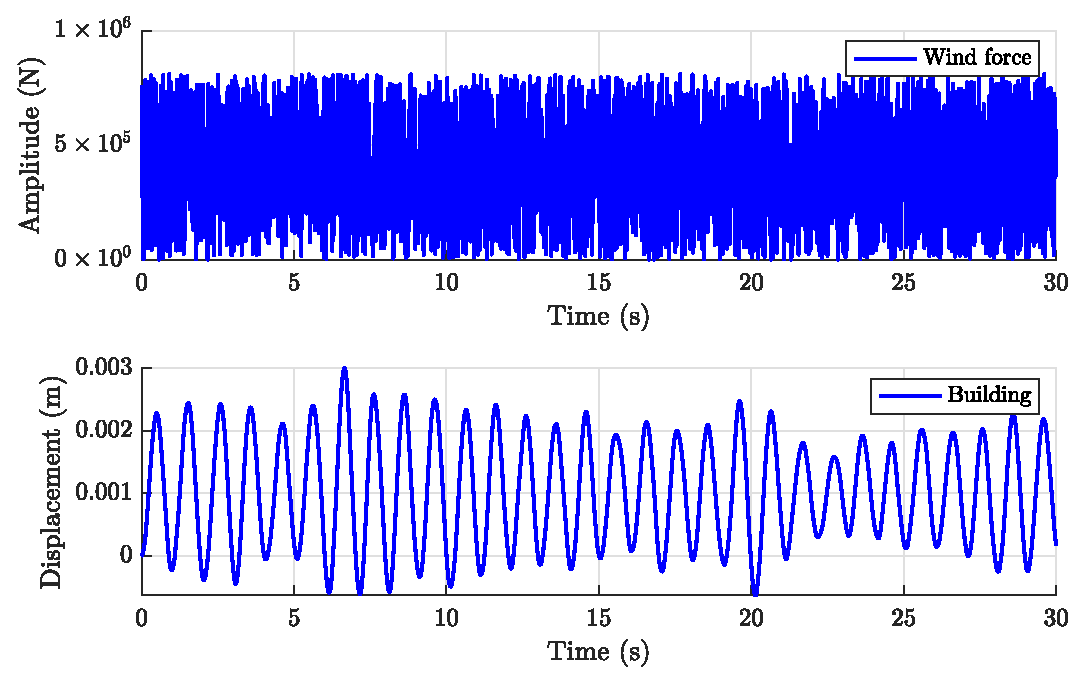
\includegraphics[width=\textwidth]{resources/eps/2_random-wind.eps}
    \caption{Open loop simulation during \SI{30}{\second} for a random wind force ($x_1=\SI{0}{\meter}$)}
\end{figure}
It can be seen that the building oscillates more or less identically and rapidly over time around a position slightly offset from its reference position.

\subsubsection{Relation with the eigenvalues and utility of a controller}
As mentioned in section \ref{sec:eigenvalues}, the eigenvalues of our system suggest that it is very reactive. Indeed, this has been observed on the different simulations : the building oscillates very quickly.\par
Eigenvalues also indicate that the system is stable. Again, this information could be found on the simulations : for a variation in initial conditions, or when the wind force is constant (or decreasing), the system tends to return to its reference position.\par
Although the movements of our building are quite small, a controller could reduce them even more, or even eliminate them completely after a while. Another role of the controller could be to slow down our system so that the building oscillates less quickly.

% Observability
\subsection{Observability}
To determine whether or not the system is observable, we computed the observability matrix thanks to Matlab function (\texttt{obsv}).\par
The matrix is full rank (verified with Matlab), the system is thus fully observable.\par
As seen on the matrix C, we need one sensor. According to the place of the non zero value, this sensor has to measure the $x_1$ state, namely the horizontal position of the top of the building $d_1$. This state is indeed the objective of the active mass damper and has thus to be observed. The sensor chosen is a position sensor (although it does not exist in that form in reality).

% Controllability
\subsection{Controllability}
To determine whether or not the system is controllable, we computed the controllable matrix thanks to Matlab function (\texttt{ctrb}). In order not to take into account the uncontrollable input (wind), only the second column of the B matrix was kept for the calculation.\par
The matrix is full rank (verified with Matlab), the system is thus fully controllable.\par
As seen on matrix B, we need only one actuator. The first column of the $B$ matrix represents the wind, while the second one concerns the damper. This latter is indeed the only controllable input and contains two non-zero elements. As a result, only one actuator is needed, and acts on two states, the speed of the building and the speed of the damper, as they take place on $x_2$ and $x_4$. The chosen actuator is a piston.

    
    % ----- Controller in time domain ----- %
    \section{Controller in time domain}

% State feedback controller
\subsection{State feedback controller}
In a first time, we need to compute the gain matrix $K$.\par
In order not to apply a gain on the wind force, the matrix K is as follows :
$$
K = \begin{pmatrix}
    0 & 0 & 0 & 0\\ 
    g_1 & g_2 & g_3 & g_4
\end{pmatrix}
$$
Indeed, the first column of matrix B concerns the uncontrollable input, so matrix K cannot affect these values.\par
The new dynamic matrix of the closed-loop system is $A_{CL} = A - BK$. Let's determine the eigenvalues of that matrix.\par
As we have a matrix of dimension $4$, the approximation of the dominant poles will be done. Indeed, we have, from the previous matrix $A$, the eigenvalues :
\begin{align*}
    \lambda_1 &= \num{-0.0634 + 6.2837i}\\
    \lambda_2 &= \num{-0.0634 - 6.2837i}\\
    \lambda_3 &= \num{-0.1666 + 1.8179i}\\
    \lambda_4 &= \num{-0.1666 - 1.8179i}
\end{align*}
As already discussed in section \ref{sec:eigenvalues}, one can see that $\lambda_3$ and $\lambda_4$ are about 10 times bigger than the last two. They are not dominant when affecting the dynamics of the system, and will therefore remain in $A_{CL}$, although slightly modified, as explained after.\par
Imposing that $(s - \lambda_3)(s - \lambda_4)$ is part of the decomposition, we get that the determinant of $A_{CL}$ is equal to :
$$
(s - \lambda_3)(s - \lambda_4)(s^2 + 2 \zeta\omega_c s + \omega_c^2) = 0
$$
Since $\lambda_3$ and $\lambda_4$ are fixed, we only need to solve the equation of the second degree in $s$ in order to find the expressions of $\lambda_1'$ and $\lambda_2'$ as a function of $\zeta$ and $\omega_c$.\par
The solutions of the equation are given by :
$$
\begin{cases}
    \lambda_1' = -\zeta\omega_c - \omega_c\sqrt{\zeta^2 - 1}\\
    \lambda_2' = -\zeta\omega_c + \omega_c\sqrt{\zeta^2 - 1}
\end{cases}
$$
The values of $\zeta$ and $\omega_c$ will be determined by simulations in the following sections. When these have been fixed, the values of the 4 poles of $A_{CL}$ will be obtained. Then we will just have to use the \texttt{place} function of Matlab to obtain the values $g_i$ of matrix $K$ associated with the eigenvalues.\par
However, as previously noted via simulations, our system is very reactive. The two non-dominant eigenvalues thus have also been modified in order to slow down the system. We finally obtain the expressions of the 4 eigenvalues of the controller :
$$
\begin{cases}
    \lambda_1' = -\zeta\omega_c - \omega_c\sqrt{\zeta^2 - 1}\\
    \lambda_2' = -\zeta\omega_c + \omega_c\sqrt{\zeta^2 - 1}\\
    \lambda_3' = \mathbb{R}(\lambda_3)0.5 + \mathbb{I}(\lambda_3)i\\
    \lambda_4' = \mathbb{R}(\lambda_4)0.5 + \mathbb{I}(\lambda_4)i
\end{cases}
$$
As the reference is 0, $k_r$ has not to be considered, so it can fixed to 0.\par
However, some tests of a change in reference will be performed in this report. We therefore calculated $k_r$ using the following formula :
$$
k_r = \frac{-1}{C(A - BK)^{-1} B}
$$
where only the controllable part of matrix B (second column) and the non-zero row of K were considered. Indeed, if the entire matrices were used, it would mean that we would have an action on the uncontrollable input, which is not possible.

% Observer
\subsection{Observer}
The controllable input being a linear combination of the different states multiplied by gains, the control system requires the different states as inputs. However, the open loop system only provides one output.\par
Considering that the real states cannot be measured in practice, the observer is a tool that allows us, based only on the output of the open loop system and on the inputs, to approximate the different states of the system.\par
Its realization must be such that the convergence of the estimated states with the real states is as fast and correct as possible.\par
One thus needs to compute the gain matrix $L$ :
$$
L = \begin{pmatrix}
    l_1\\
    l_2\\
    l_3\\
    l_4
\end{pmatrix}
$$
The new dynamic matrix is given by $A_{obs} = A - LC$.\par
As previously, we will keep the same two non-dominant eigenvalues and determine the two other via the same method that has been used for $K$.\par
Imposing that $(s - \lambda_3')(s - \lambda_4')$ is part of the decomposition, we get that the determinant of $A_{obs}$ is equal to :
$$
(s - \lambda_3')(s - \lambda_4')(s^2 + 2 \zeta\omega_c s + \omega_c^2) = 0
$$
Since $\lambda_3'$ and $\lambda_4'$ are fixed, we only need to solve the equation of the second degree in $s$ in order to find the expressions of $\lambda_1^*$ and $\lambda_2^*$ as a function of $\zeta$ and $\omega_c$.\par
The solutions of the equation are given by :
$$
\begin{cases}
    \lambda_1^* = -\zeta\omega_c - \omega_c\sqrt{\zeta^2 - 1}\\
    \lambda_2^* = -\zeta\omega_c + \omega_c\sqrt{\zeta^2 - 1}
\end{cases}
$$
The poles of the observer are determined by taking the poles of the controller and moving them. To do this, the real parts of each pole are multiplied by a constant $\alpha$. In the case of poles $\lambda_1'$ and $\lambda_2'$, this amounts to multiplying $\omega_c$ by $\alpha$.\par
We finally have :
$$
\begin{cases}
    \lambda_1^* = -\zeta\omega_c\alpha - \omega_c\alpha\sqrt{\zeta^2 - 1}\\
    \lambda_2^* = -\zeta\omega_c\alpha + \omega_c\alpha\sqrt{\zeta^2 - 1}\\
    \lambda_3^* = \mathbb{R}(\lambda_3')\alpha + \mathbb{I}(\lambda_3')i\\
    \lambda_4^* = \mathbb{R}(\lambda_4')\alpha + \mathbb{I}(\lambda_4')i
\end{cases}
$$
The values $l_i$ of the matrix $L$ are then obtained by using the \texttt{place} function of Matlab. The chosen values are given in the next section.

% Simulations and discussion
\subsection{Simulations and discussion}
\subsubsection{Parameter determination}
In order to best achieve our control system, we must determine the values of $\zeta$, and $\omega_c$. We know that the system control is done via the controllable input $u(t)$, and that this input will influence the variation of the output and the different states of the system.\par
In order to obtain a coherent system, {\it i.e.} physically possible state values and an attenuation of building oscillations, we must choose values of $\zeta$ and $\omega_c$ that will lead to a control input making the system coherent.\par
We tested several values of $\zeta$ as well as several values of $\omega_c$ with a constant wind force~:
\begin{figure}[H]
    \centering
    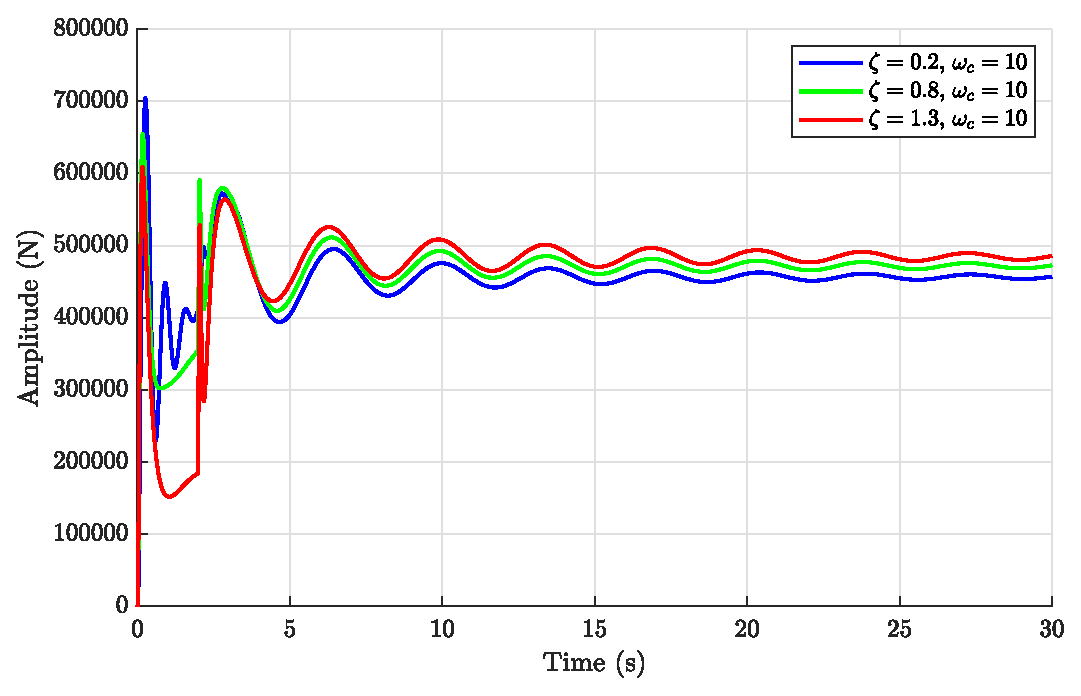
\includegraphics[width=\textwidth]{resources/eps/3_zeta-variations.eps}
    \caption{Control input $u(t)$ for different variations of parameter $\zeta$}
\end{figure}
\begin{figure}[H]
    \centering
    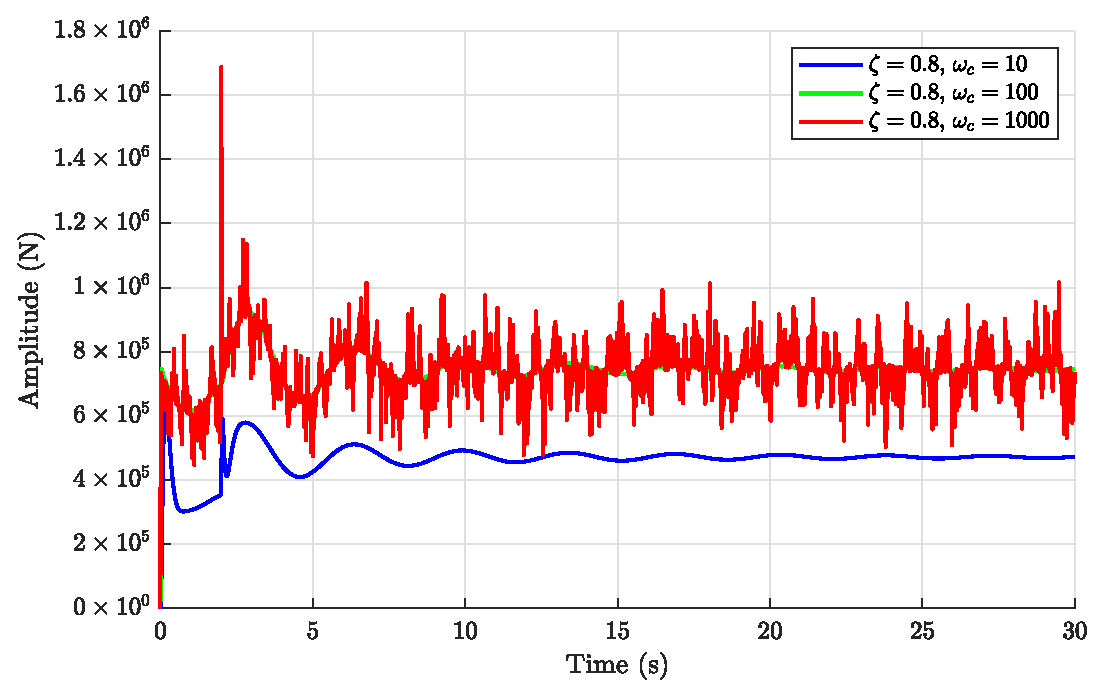
\includegraphics[width=\textwidth]{resources/eps/3_omega-variations.eps}
    \caption{Control input $u(t)$ for different variations of parameter $\omega_c$}
\end{figure}
It can be seen that the variations in parameter $\zeta$ have little influence on the controllable force : after a few seconds, it is identical in all cases.\par
Concerning the parameter $\omega_c$, we observe that the higher it is, the faster the control force oscillates (which is an undesirable behaviour).\par
We also observed the variation of the parameter $\omega_c$ on the states $x_1$ (also the output) and $x_3$ of our system :
\begin{figure}[H]
    \centering
    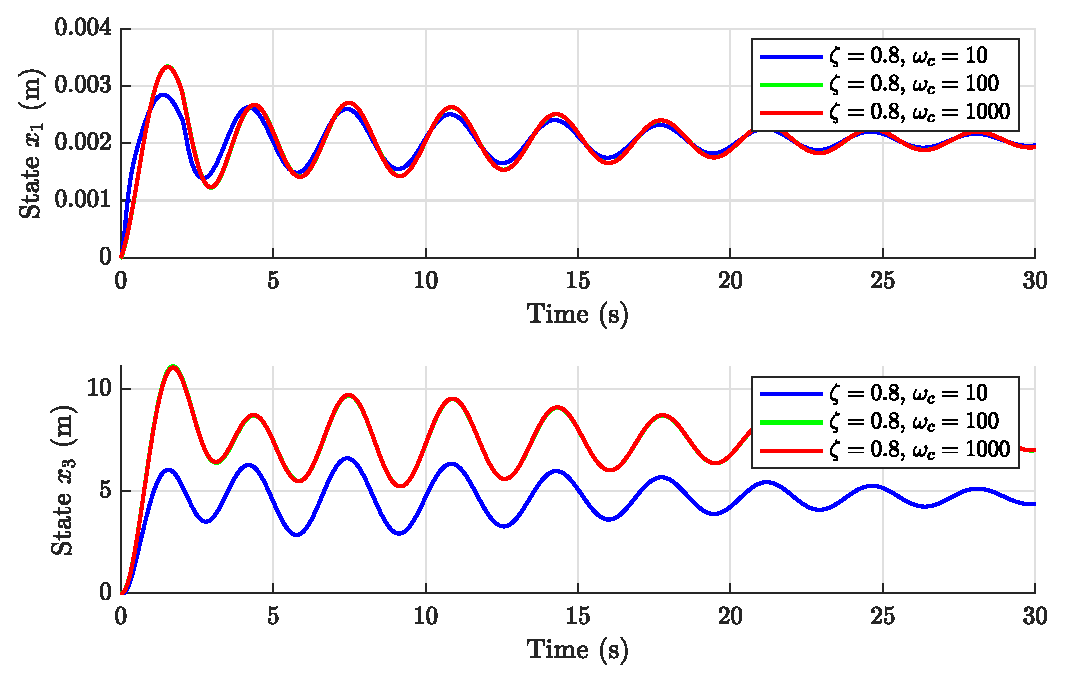
\includegraphics[width=\textwidth]{resources/eps/3_states-variations.eps}
    \caption{States $x_1$ and $x_3$ of the system for different variations of parameter $\omega_c$}
\end{figure}
First of all, we observe that the green and red curves overlap perfectly. Then, we find that the influence of the $\omega_c$ parameter on the states is relatively small. Only the damper's behaviour varies considerably.\par
The variations of the $x_2$ and $x_4$ statements are very similar and lead to the same observations.\par
The parameter $\zeta$ has little influence on the controllable input, so the variations of the states according to its different values are also small and we have chosen not to highlight them in this report.\par
We also checked the influence of these parameters on a variation of the reference and on a noisy input. The observations are identical to those made on the statements (slight variations for $\omega_c$ and some slight variations for $\zeta$).\par
We therefore choose to take the following values of the parameters :
$$
\begin{cases}
    \zeta = \num{0.8}\\
    \omega_c = \num{10}
\end{cases}
$$
We also arbitrarily choose our parameter $\alpha = 5$. This choice, in regards of the simulations presented later, is proving to be a good one.\par
These values allowed us to calculate the eigenvalues of the matrices $A_{CL}$ and $A_{obs}$ and thus to obtain our matrices $K$ and $L$ :
$$
\begin{cases}
    \lambda_1' = \num{-8.0000 + 6.0000i}\\
    \lambda_2' = \num{-8.0000 - 6.0000i}\\
    \lambda_3' = \num{-0.0833 + 1.8179i}\\
    \lambda_4' = \num{-0.0833 - 1.8179i}
\end{cases}
\quad
\begin{cases}
    \lambda_1^* = \num{-3.3057}\\
    \lambda_2^* = \num{0.0734}\\
    \lambda_3^* = \num{0.0064 + 0.0259i}\\
    \lambda_4^* = \num{0.0064 - 0.0259i}
\end{cases}
$$
With these different values, our control input is as follows :
\begin{figure}[H]
    \centering
    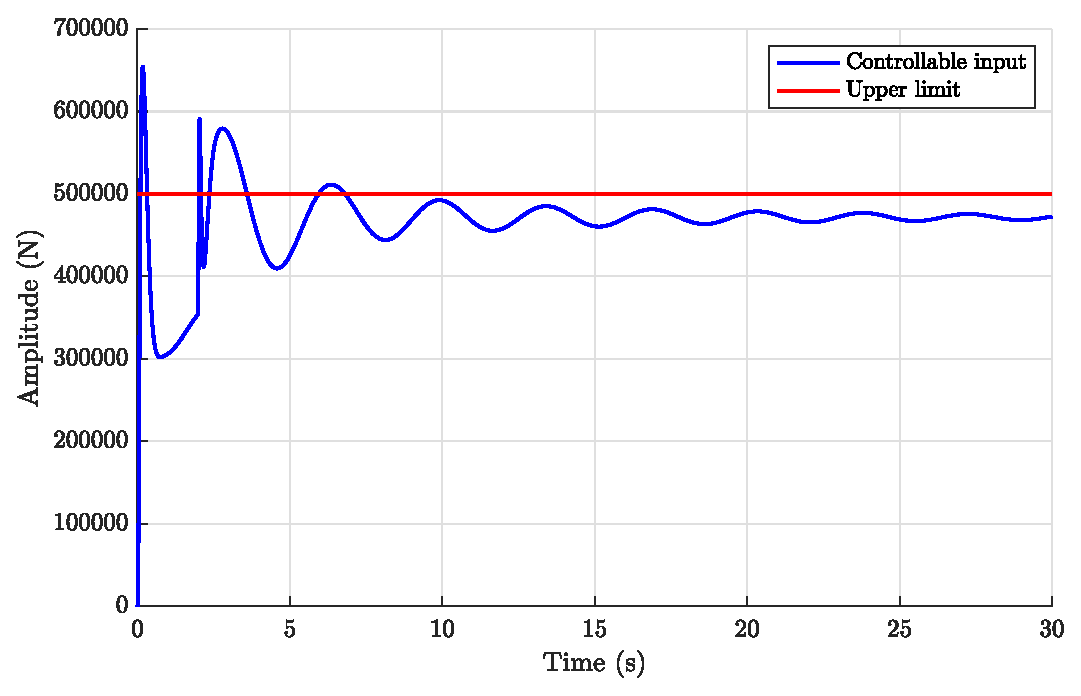
\includegraphics[width=\textwidth]{resources/eps/3_controllable-input.eps}
    \caption{Control input $u(t)$ for $\zeta = \num{0.8}$ and $\omega_c = \num{10}$}
\end{figure}
An abnormally high peak is observed at the beginning. This peak is due to the unrealistic simulations performed : the simulation goes from a zero wind to a constant wind of several thousand newtons in an instant (similar to a step). However, it can be seen that after this peak, the control force oscillates around much more realistic values within our previously defined acceptable range of values.\par
This control input does allow a reduction in building oscillations, and this in a relatively slower way (the system has been slowed down).
\begin{figure}[H]
    \centering
    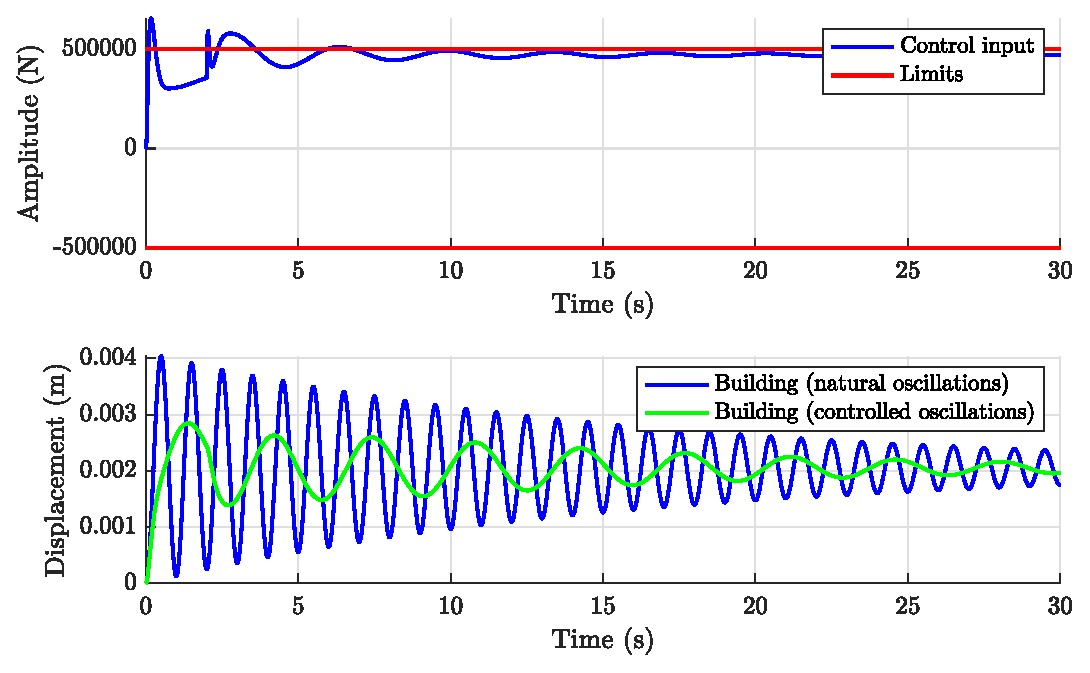
\includegraphics[width=\textwidth]{resources/eps/3_constant.eps}
    \caption{System simulation with and without control input for a constant wind.}
    \label{fig:3.controller}
\end{figure}
We can now evaluate the performance of our observer. To do this, we launched a 10-second simulation with a sinusoidal wind force. In order to observe its convergence, the controlled system and observer have different initial conditions and a time delay upon entry (\SI{2}{\second}).
\begin{figure}[H]
    \centering
    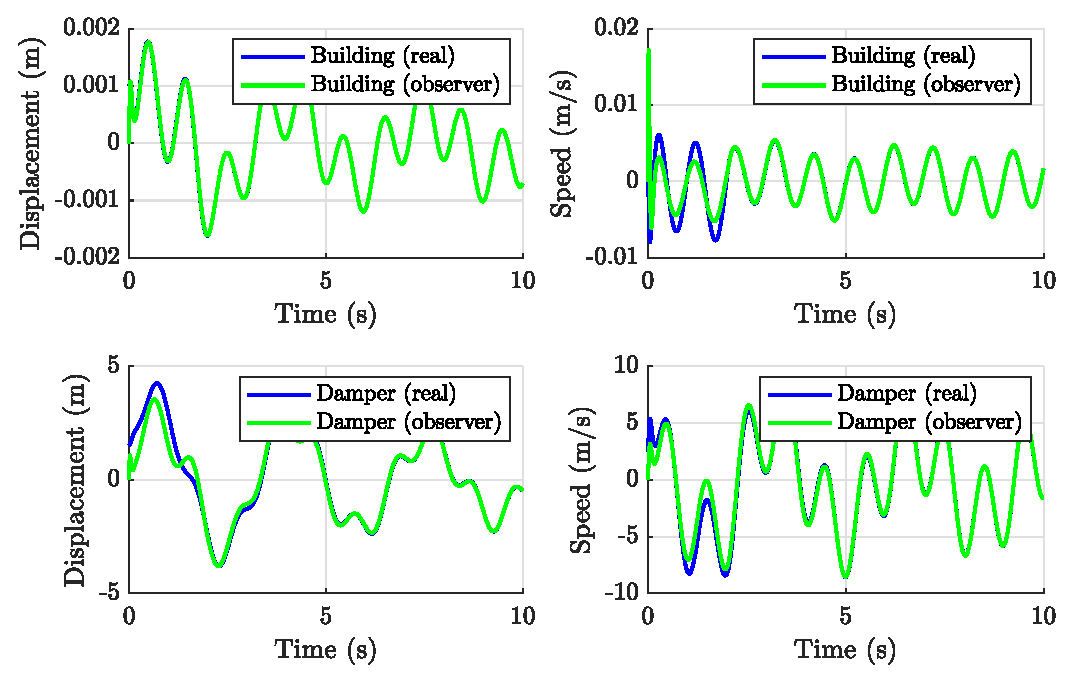
\includegraphics[width=\textwidth]{resources/eps/3_observer.eps}
    \caption{Simulation of the observer with a sinusoidal wind force}
\end{figure}
We notice that our observer converges very quickly (5 seconds maximum, 10 for absolute convergence) towards the real states of the system. Its realization seems to be correct.\par
We can also see that the values of our states, with the control system in place, seem to be consistent and within the plausible value domains we defined earlier.\par
We will now study the behaviour of the system in several situations. We have not plotted the influence of $\zeta$ and $\omega$ as they have an almost identical behaviour as for the previous discussions that led to their determination.

\subsubsection{Response to a reference variation}
For this simulation, we have set the uncontrollable input to 0 and changed the reference to \SI{0.002}{\meter}.
\begin{figure}[H]
    \centering
    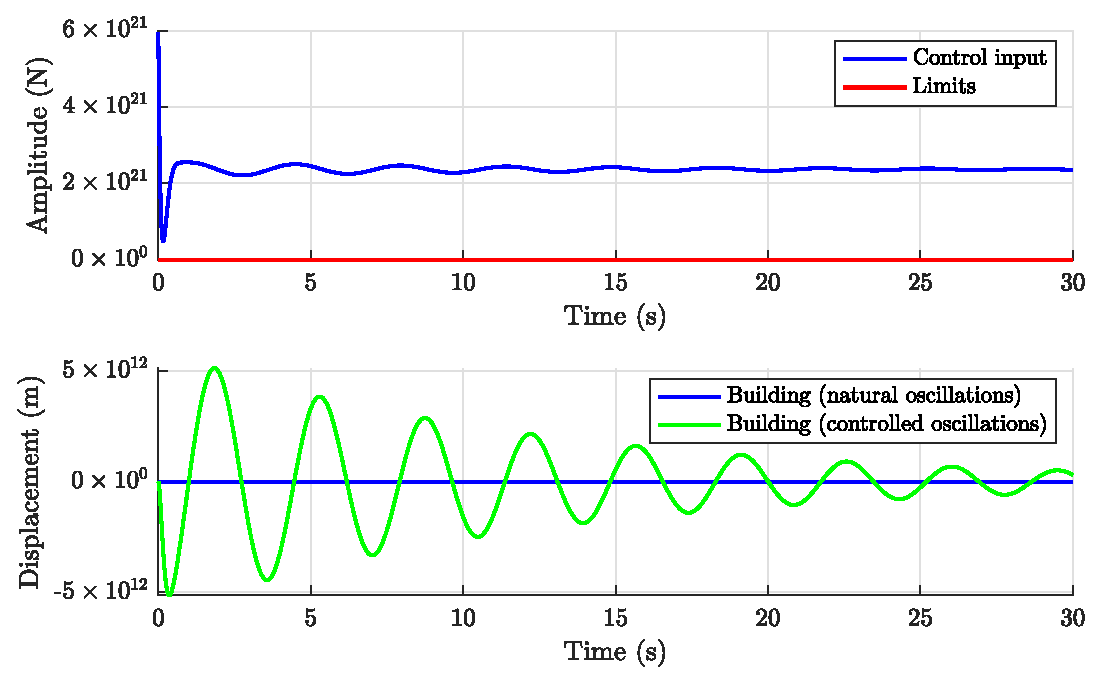
\includegraphics[width=\textwidth]{resources/eps/3_reference.eps}
    \caption{System simulation with a reference variation of \SI{0.002}{\meter}}
\end{figure}
We observe that the values of the controlled signal are totally incoherent. We have not found where this problem comes from. We have designed $k_r$ so that the system is robust to reference variations. The expected behaviour is therefore not normal nor intended.\par
However, the reference of our building is not supposed to change over time, and being resistant to that kind of change is not something we think is needed for this instance.

\subsubsection{Response to a perturbation (disturbance)}
We simulated our different wind scenarios to see how the controlled system reacts. The constant wind scenario has already been presented in figure \ref{fig:3.controller}. We therefore simulated the two remaining scenarios.
\begin{figure}[H]
    \centering
    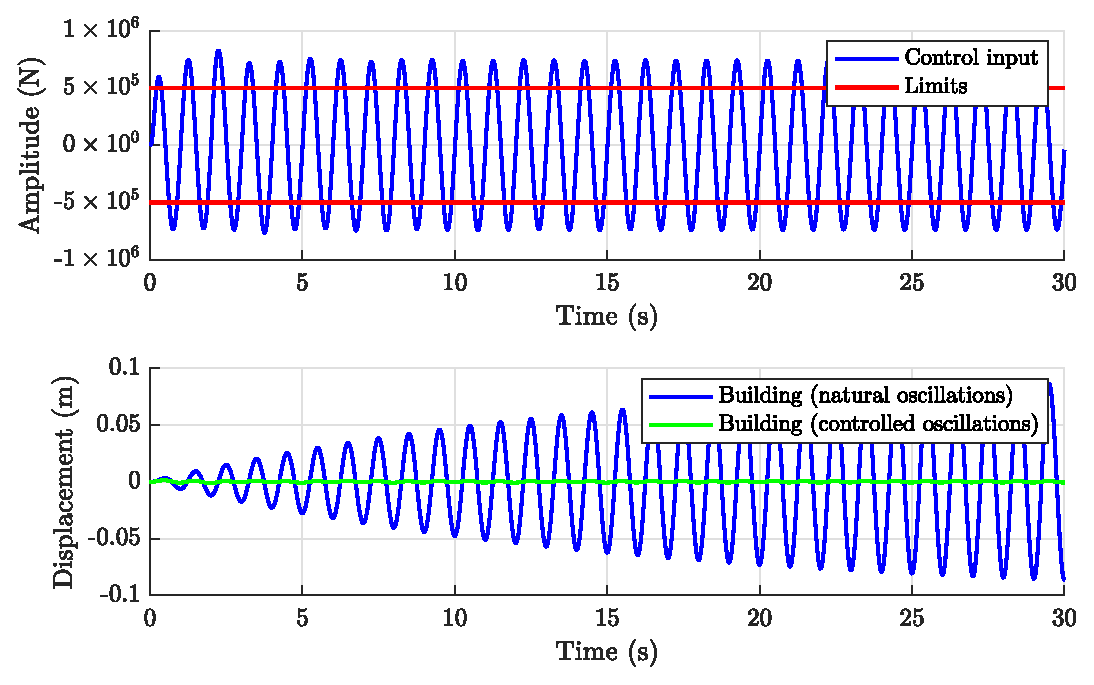
\includegraphics[width=\textwidth]{resources/eps/3_sinusoidal.eps}
    \caption{System simulation with a sinusoidal wind force}
\end{figure}
\begin{figure}[H]
    \centering
    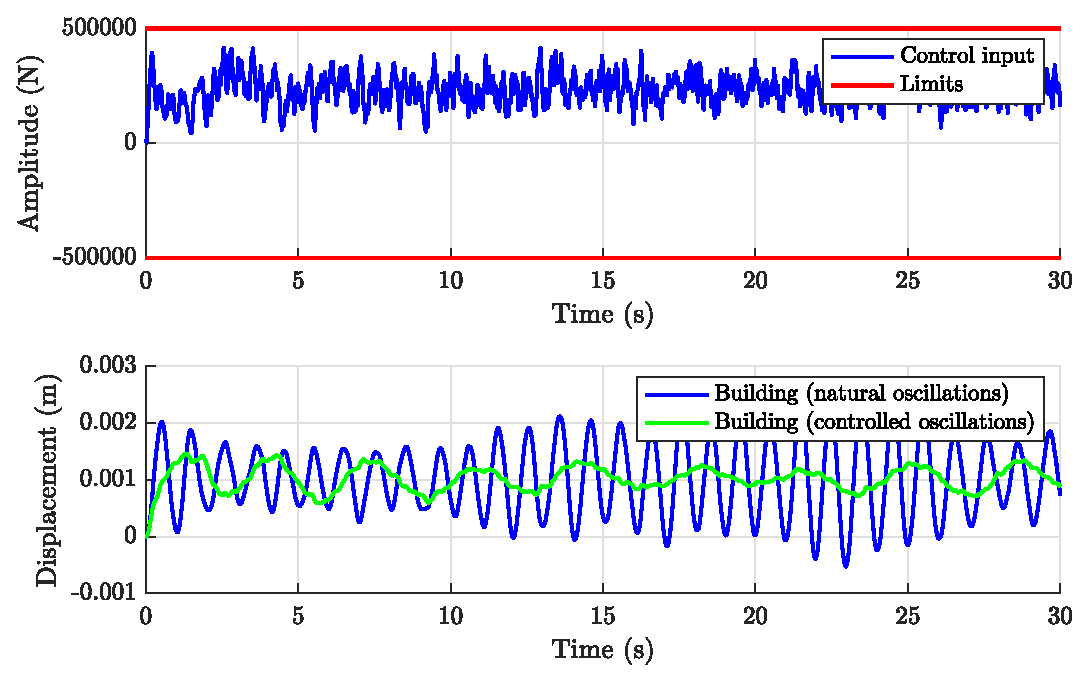
\includegraphics[width=\textwidth]{resources/eps/3_random.eps}
    \caption{System simulation with a random wind force}
\end{figure}
For each of the scenarios, we can see that the oscillations of the buildings are attenuated and tend to disappear completely quite quickly. The controlled system is much slower than the initial system.\par
Our control therefore seems to be fulfilling its role well, although the force we need to apply to our controller is sometimes a bit too high compared to our constraints. We have spent hours trying to reach these constraints by tweaking the parameters of our controller, but this is the best we could manage. More information on that is given in the general conclusion.

\subsubsection{Presence of noise}
For this simulation, we added a random noise (approximately 5\% of the nominal value) to the inputs of the observer (so the output of the controller and the delayed disturbance of the observer). This noise will influence the control input, and therefore the system output.\par
The control input affected by noise is shown in figure \ref{fig:3.noise.control.input}.
\begin{figure}[H]
    \centering
    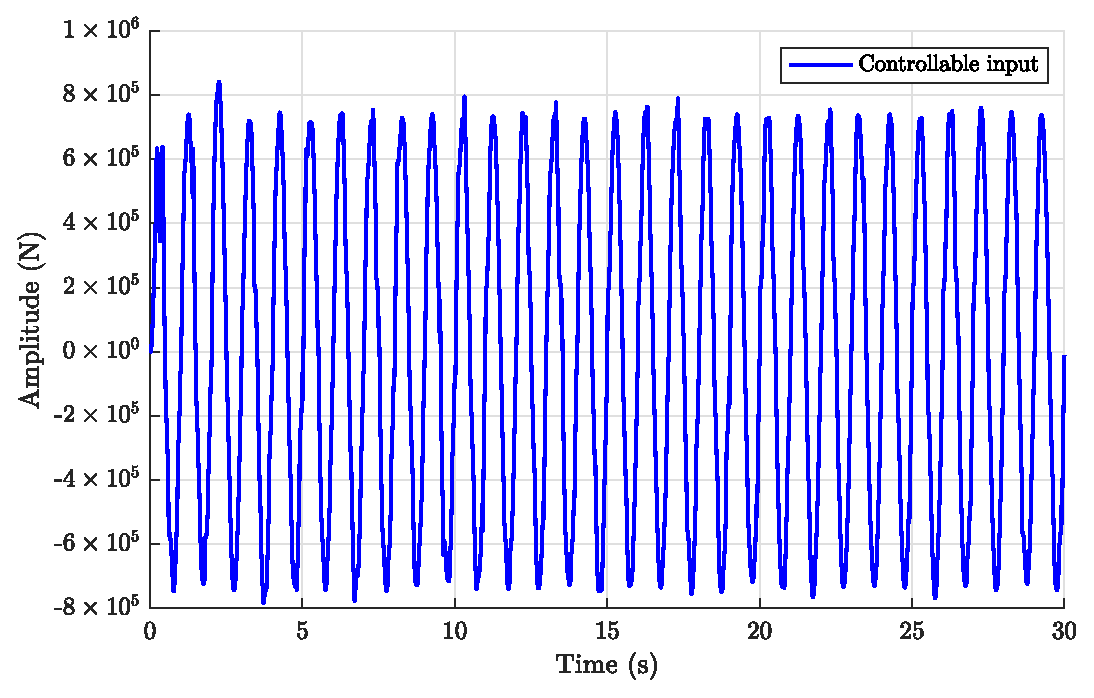
\includegraphics[width=\textwidth]{resources/eps/3_noise-controllable-input.eps}
    \caption{Control input $u(t)$ with noise in the observer}
    \label{fig:3.noise.control.input}
\end{figure}
The system output (as well as the original disturbance) is shown in figure \ref{fig:3.noise}.
\begin{figure}[H]
    \centering
    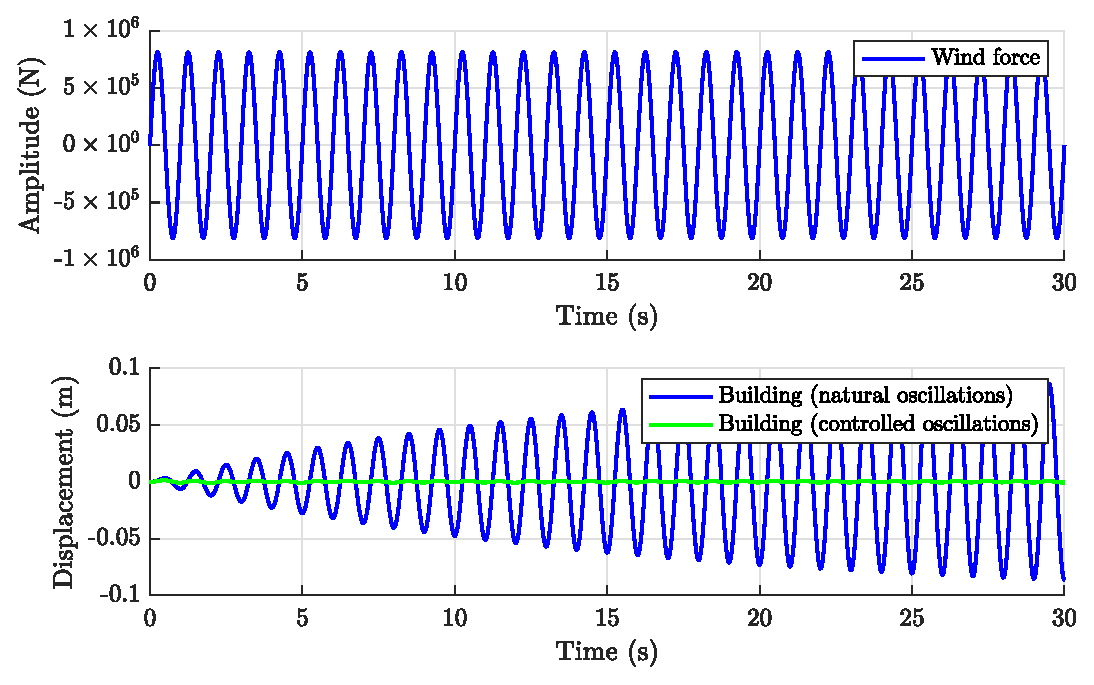
\includegraphics[width=\textwidth]{resources/eps/3_noise.eps}
    \caption{System simulation with noise in the observer}
    \label{fig:3.noise}
\end{figure}
We see that our system is robust to noise. Indeed, despite the presence of the latter, the building's oscillations are still very well attenuated. A try for an explanation is given in the general comparison between the two controllers.

    
    % ----- Controller in frequency domain ----- %
    \section{Controller in frequency domain}

% Framework
\subsection{Framework}
For this part of the work, it has decided to simplify our system and use 2 states instead of 4. The position and speed of the damper are therefore hidden in the force of the actuator, which is still the controllable input of the system.
\begin{figure}[H]
    \centering
    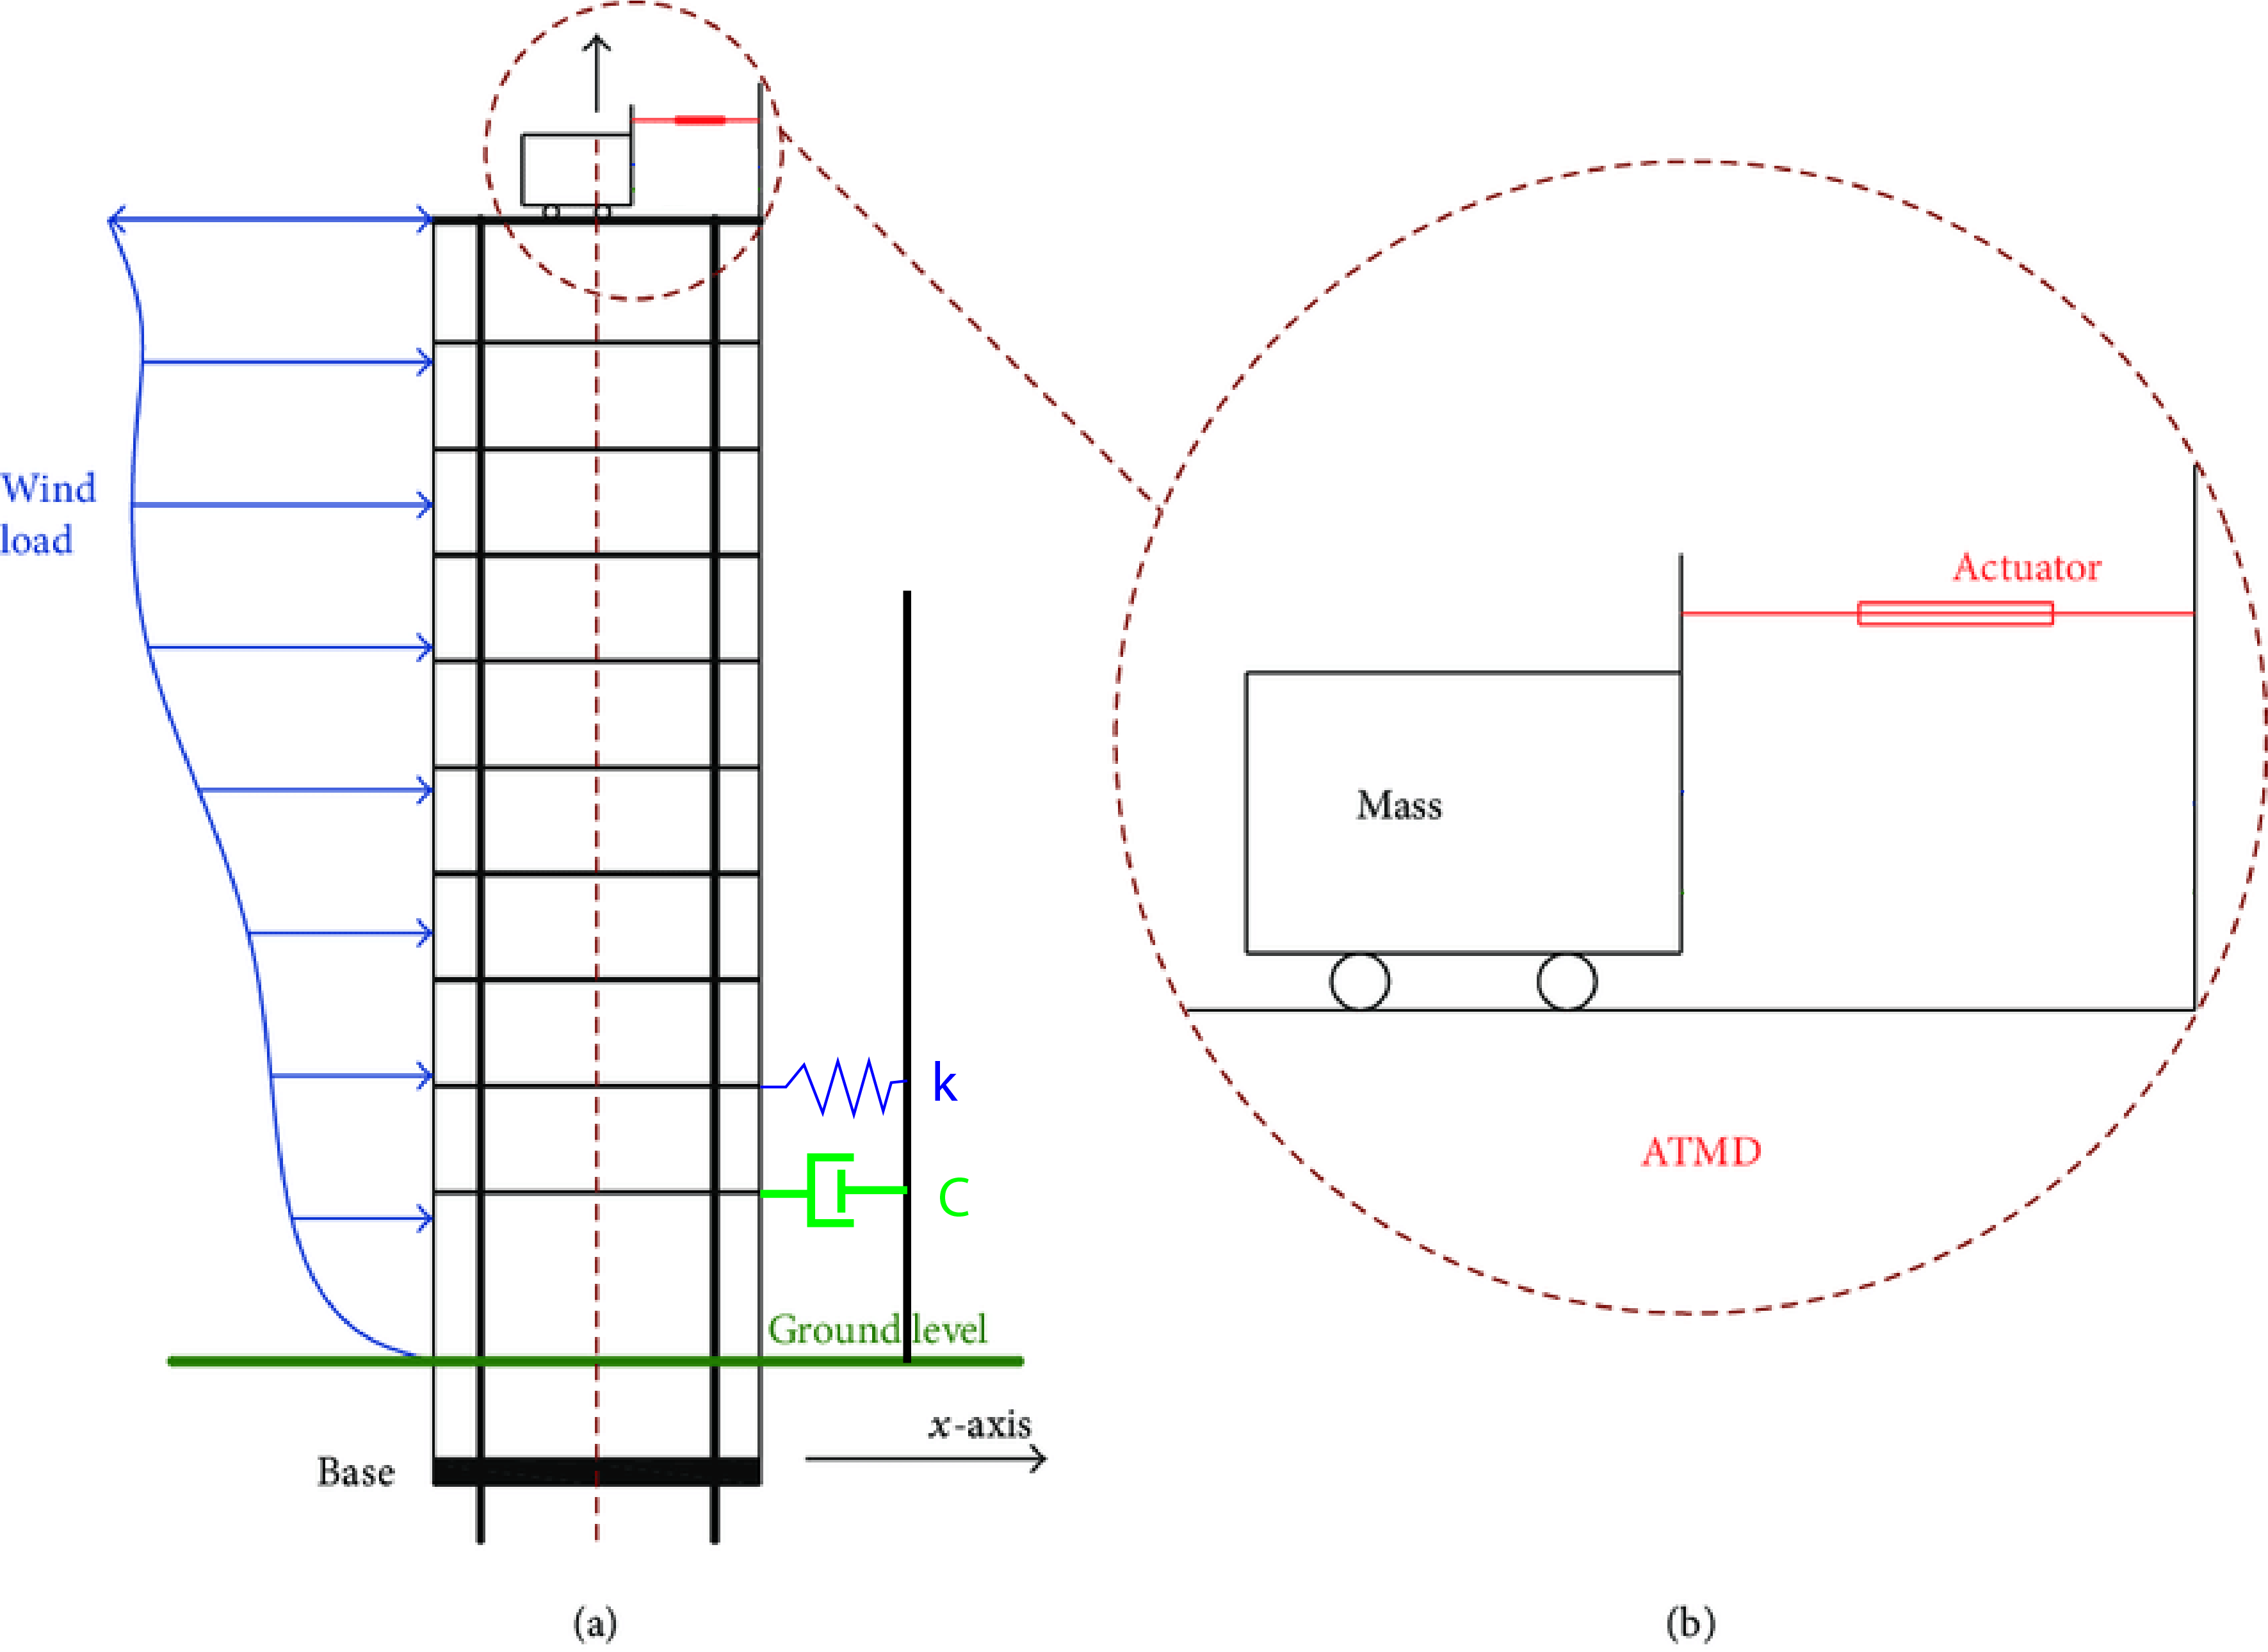
\includegraphics[width=0.7\textwidth]{resources/png/4_simplified-system.png}
    \caption{Simplified system of an active mass damper}
    \label{fig:simplified-system}
\end{figure}
The law that governs that system is the following : 
$$
m_{tot}\ddot{x} + c\dot{x} + kx = F_{wind} + F_{damper}
$$
where
\begin{itemize}
    \item $F_{damper} = m_{damper}a_{damper}$
    \item $m_{tot} = m_{building} + m_{damper}$
    \item $x$ is the position of the building relative to its rest position ($x = 0$)
\end{itemize}
Let's now define the input, output and states : 
\begin{itemize}
    \item $u_1 = F_{wind}$
    \item $u_2 = F_{damper}$
    \item $x_1 = x$
    \item $x_2 = \dot{x}$
    \item $y = x_1$ 
\end{itemize}
By doing so, the ABCD matrices are the following :
$$
A = \begin{pmatrix}
    0 & 1\\
    \dfrac{-k}{m_{tot}} & \dfrac{-c}{m_{tot}}\\
\end{pmatrix}
\quad
B = \begin{pmatrix}
    0 & 0\\
    \dfrac{1}{m_{tot}} & \dfrac{1}{m_{tot}}\\
\end{pmatrix}
$$
$$
C = \begin{pmatrix}
    1 & 0\\
\end{pmatrix}
\quad
D = \begin{pmatrix}
    0 & 0\\
\end{pmatrix}
$$

\subsubsection{Constraints and simulation specifications}
We have the following constraints : 
\begin{itemize}
    \item Acceleration of the mass damper below \num{1.6}$g$, to be consistent with the time domain.
    \item Lateral movement of the top of the building not above \SI{1}{\meter}.
\end{itemize}
The two scenarios we look at are the following : a turbulent wind of maximum \SI{810}{\kilo\newton}, that is represented as a sine function and a constant wind of the same intensity (the random wind has been studied and is referenced but is not plotted for this section).\par
Here are the values of the different parameters that have been chosen, as previously : 
\begin{table}[H]
    \centering
    \begin{tabular}{|l|c|c|}
        \hline
        {\bf Mass} & $m_{building} = \SI{1e7}{\kilogram}$ & $m_{damper} = \SI{3e4}{\kilogram}$\\ \hline
        {\bf Spring} & \multicolumn{2}{c|}{$k\approx\SI{4e8}{\newton\per\meter}$}\\ \hline
        {\bf Damper} & \multicolumn{2}{c|}{$c\approx\SI{1.3e6}{\newton\second\per\meter}$}\\ \hline
        {\bf Wind} & \multicolumn{2}{c|}{$F_{max} = \SI{810}{\kilo\newton}$}\\ \hline
    \end{tabular}
    \caption{Numerical values of the system}
    \label{tab:numerical-values}
\end{table}

\subsubsection{Choice of cross-over frequency}
The frequency of the building is of about \SI{1}{\hertz}, as advised by Pr. Denoël, and the frequency of the sinusoidal wind studied is also of \SI{1}{\hertz}. So the cross-over frequency was initially set at \SI{5}{\hertz}.\par
All frequencies above that, probably coming from noise and unwanted phenomena, will be attenuated, while the amplitudes of the frequencies below that, which correspond to the internals of the system, will be amplified.\par
In the end, after some simulations, we have decided to put the crossover frequency at \SI{20}{\radian\per\second} as we have found out that a smaller crossover frequency induces a slightly slower response in our system. Although not noticeable in the sinusoidal force scenario, it can be seen when the disturbance is a constant or a random function.

% Transfer function of the open-loop system
\subsection{Transfer function of the open-loop system}
\subsubsection{Computation}
For the computation of the transfer function of our system, we used the Matlab function \texttt{tf(sys)} then selecting the answer corresponding to our controllable input. In our case,
$$
P(s) = \dfrac{9.97e-8}{s^2 + 0.1257s + 39.48}
$$
Had we wanted to compute it by hand, we would have translated our ABCD system to its frequency form (derivative becomes a multiplication by $s$), then we would have found that
$$
H(s)=\frac{Y(s)}{U(s)}=C(s I-A)^{-1} B+D
$$
By selecting only the columns of B and D corresponding to the controllable input, we would have found the same expression as the one above.

\subsubsection{Plots}
The Bode plots of the open-loop system are given at figure \ref{fig:bode-ol}.
\begin{figure}[H]
    \centering
    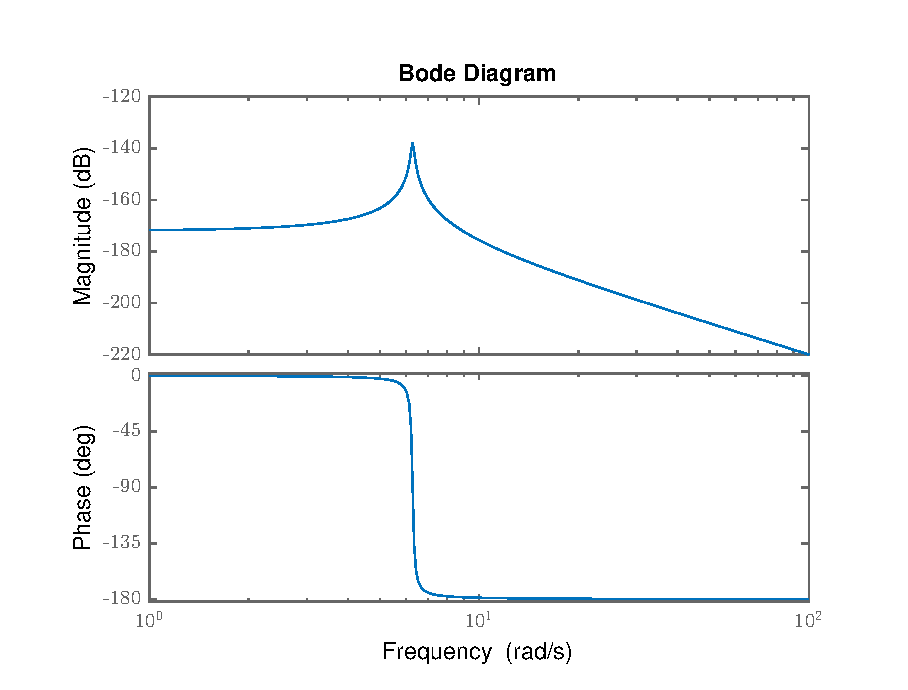
\includegraphics[scale=0.8]{resources/eps/4-Val/bode-ol.eps}
    \caption{Bode plots for 2D system}
    \label{fig:bode-ol}
\end{figure}
These graphs have the typical shape of the second order systems. If we confront our transfer function with the typical transfer function of such a system ($H(s)=\frac{1}{s^{2}+2 \zeta \omega_{n} s+\omega_{n}^{2}}$), we find that $\omega_n\approx6.28$ and $\zeta \approx 0.01$.\par
We thus have two complex poles, oscillations and overshoots. The peak is quite high, as $\zeta \ll 1$, and the transition from \SI{0}{\degree} to \SI{-180}{\degree} (at $\omega_n$, the natural frequency of our system) is quite sharp for the same reasons.

% Loop shaping
\subsection{Loop shaping}
\subsubsection{Lag compensator}
Firstly, we have decided to use a lag compensator in order to increase the gain for low frequencies (remove the flat area at low frequencies) and thus have a better response. We have used a lag compensator of the following shape :
$$
Glag(s) = \dfrac{s + a}{s}
$$
The bode diagram of that transfer function is given at figure \ref{fig:glag}.
\begin{figure}[H]
    \centering
    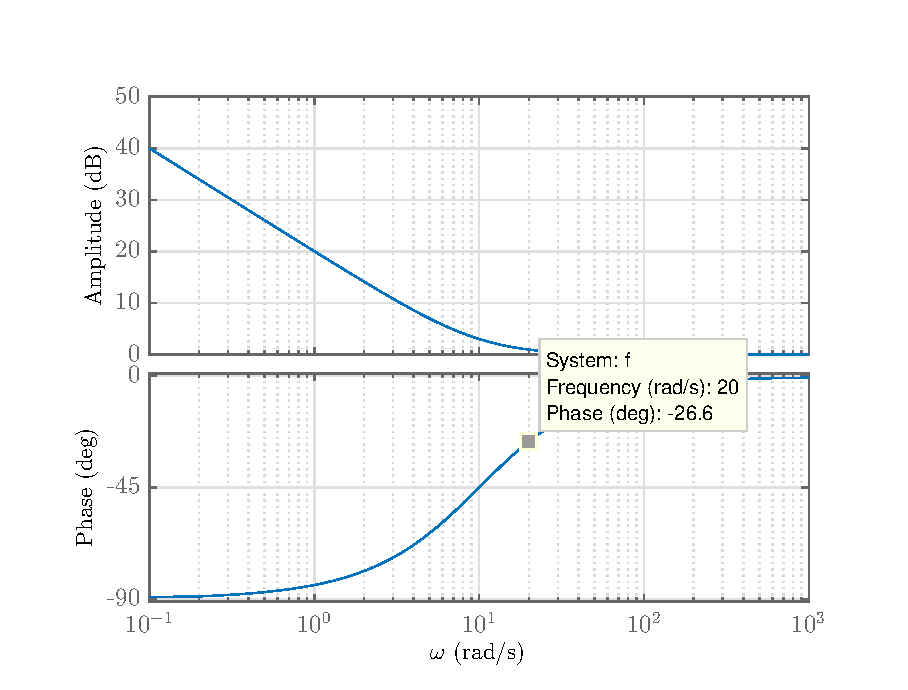
\includegraphics[scale = 0.8]{resources/eps/4-Val/glag.eps}
    \caption{Bode diagrams of the lag compensator}
    \label{fig:glag}
\end{figure}
We have decided to use a $a$ of $10$ to attenuate the natural frequency spike in the initial Bode amplitude diagram without interfering too much with the phase diagram ($a$ is used to move the point at which the amplitude of the Bode diagram becomes \SI{0}{\deci\bel}).\par
As can be seen, this element induces a phase of about \SI{-26}{\degree} at the crossover frequency, but it is not a problem as we have succeeded in tuning our lead compensator to be resistant to the delays we will have in our system. It can be noted that, for a sinusoidal wind, the use of such a component is not necessary. However, when we conducted tests with a constant wind (equivalent to a step), we have found out that using a lag compensator induces no static error while not using one induces a stabilization at a position different from the reference.\par
However, the acceleration of the damper becomes twice as large as those with no lag compensator. We have decided to keep it to comply with the theoretical shape of the desired Bode diagram but, in practice, if the acceleration is too intense with such a component, we could easily remove it without bringing instabilities in the response of the building.

\subsubsection{Lead compensator}
Let's now add a lead compensator to obtain the desired phase margin. Delays are discussed after, but we want to be able to respond at least to \SI{0.02}{\second} delays, which correspond to the \SI{50}{\hertz} of the actuator's piston \cite{Hassan_2016}.\par
We have finally decided to use a phase margin of \SI{80}{\degree} for the following computations, although it will translate in practice to a phase margin of \SI{42}{\degree} because of interference with the lag compensator and the low-pass filter. In order to increase the phase margin at the crossover frequency, we have decided to use a lead compensator.\par
Its transfer function is given by : 
$$
G(s) = \dfrac{\frac{s}{w_z} + 1}{\frac{s}{w_p} +1}
$$
For a given crossover frequency $\omega_{co}$ and a phase margin $\phi_m$, we can determine the two $w$ (further apart means a phase and amplitude modifications in $L$ more spread) in the following way : 
$$
\left\{\begin{array}{l}
    {w_{z}=\tan (\alpha) w_{\mathrm{co}}} \\
    {w_{p}=\frac{w_{\mathrm{co}}}{\tan (\alpha)}}
\end{array}\right.
$$
with $\alpha = \frac{\pi}{4} - \frac{\phi_m}{2}$.\par
For the crossover frequency and the desired value of $\phi_m$, we have that that : 
$$
w_z = \num{1.75} \qquad w_p = \num{228.6}
$$
We have chosen that phase margin because, with one below \SI{65}{\degree}, the delays we have determined bring instability to our system, as we have seen in the Nyquist diagrams. Any value above that is fine in that regards and does not impact our output and controllable input in a very determinant way. However, lower phase margins tend to slightly increase the speed of our control system, so we have chosen this phase margin of \og{}\SI{80}{\degree}\fg{}. The Bode plots of this component is given at figure  \ref{fig:glead}.
\begin{figure}[H]
    \centering
    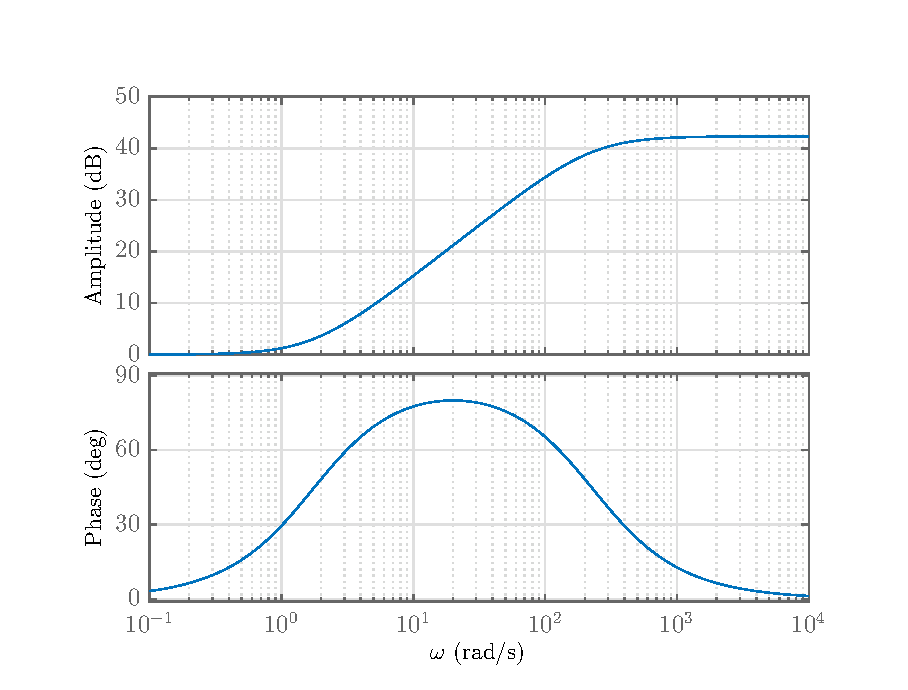
\includegraphics[scale = 0.8]{resources/eps/4-Val/glead.eps}
    \caption{Bode diagrams of the lead compensator}
    \label{fig:glead}
\end{figure}

\subsubsection{Gain}
After that, one needs to add a gain to our system in order to increase the amplitude gains for all frequencies and make it so that the amplitude is at \SI{0}{\deci\bel} at the crossover frequency. That is done by using a constant gain. This does not affect the phase but increases the amplitudes of about \SI{175.5}{\deci\bel}, which positions our Bode plot to where one wanted it to be. 

\subsubsection{Low-Pass Filter}
$$
G(s) = \dfrac{1}{\frac{s}{a}+1}
$$
We have decided to use a low-pass filter in order to attenuate even more the gains for higher frequencies.\par
In the case of a random wind, we have seen that it reduces a bit the spikes in the controllable input, so we have decided to keep it, although its action for other scenarios was not perceived. However, such a filter is designed to attenuate the effect of noise on the system, and in that regards, it works quite well with our system, as we can see in the section dedicated to noise at the end of this report.\par
As can be seen on the Bode diagrams at the figure \ref{fig:lpf}, we induce a loss in phase of about \SI{11}{\degree} by choosing a parameter $a = 5*\omega_{co}$ for the low-pass filter. However, as it has already been said for the lag compensator, the system can still react well to the delays we have identified. If it did not, we could use a bigger $a$, but we would react less nicely to noise.
\begin{figure}[H]
    \centering
    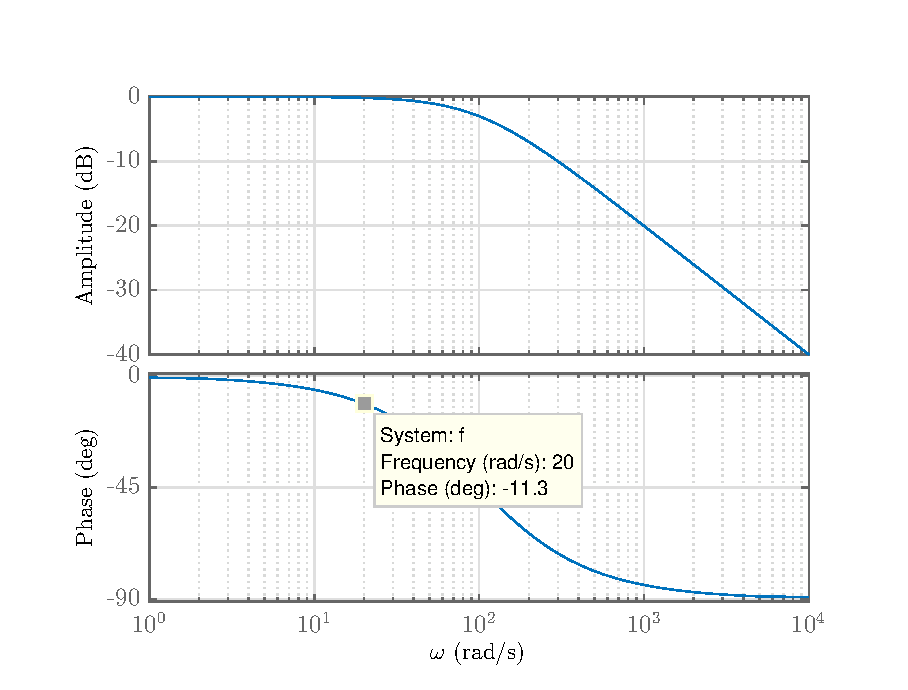
\includegraphics[scale = 0.8]{resources/eps/4-Val/lpf.eps}
    \caption{Bode diagrams of the low-pass filter}
    \label{fig:lpf}
\end{figure}

\subsubsection{Trade-offs}
The Bode and Nyquist plots of the controlled system are given at figures \ref{fig:bode-control} and \ref{fig:nyquist-control}. The different tradeoffs that had to be made are explicited in the different sections concerning the components we have used. We had to make compromises for the phase margin, the rejection of noise and the use of a lag compensator.\par
Concerning the output and the controllable input (Figures \ref{fig:controllable-input} and \ref{fig:output}, \ref{fig:controllable-input2} and \ref{fig:output2}), we can see that the damping is very well obtained, although the force needed for the damper is a bit over what we have used in our constraints (not using a lag compensator brings us below them in the case of a constant wind but not in the case of a sinusoidal one). We have tried numerous changes in parameters to go below these constraints for the sinusoidal wind but have not succeeded.
\begin{figure}[H]
    \centering
    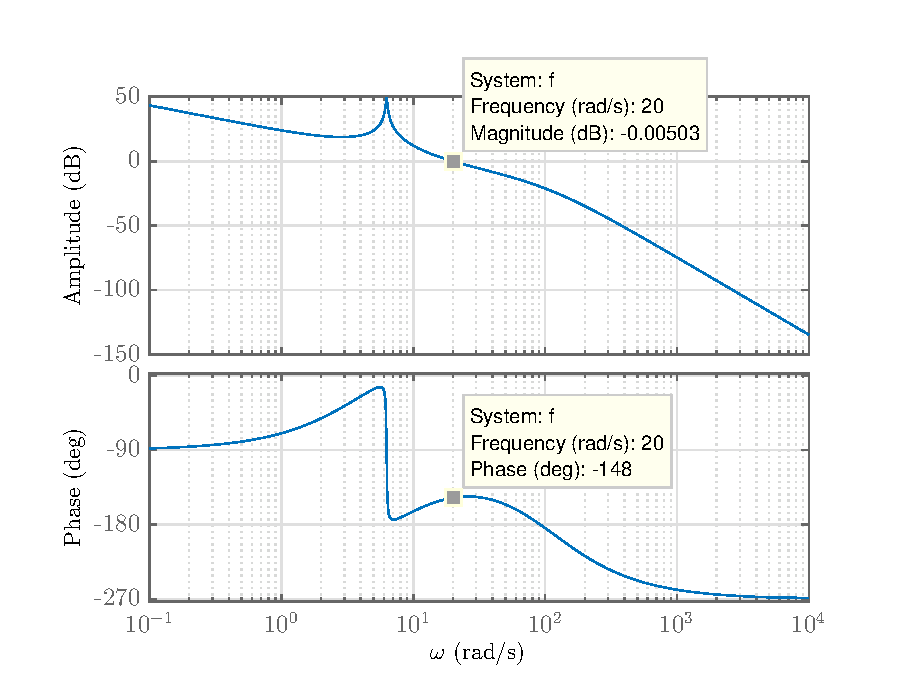
\includegraphics[scale = 0.8]{resources/eps/4-Val/L.eps}
    \caption{Bode plots of the controlled system}
    \label{fig:bode-control}
\end{figure}
\begin{figure}[H]
    \centering
    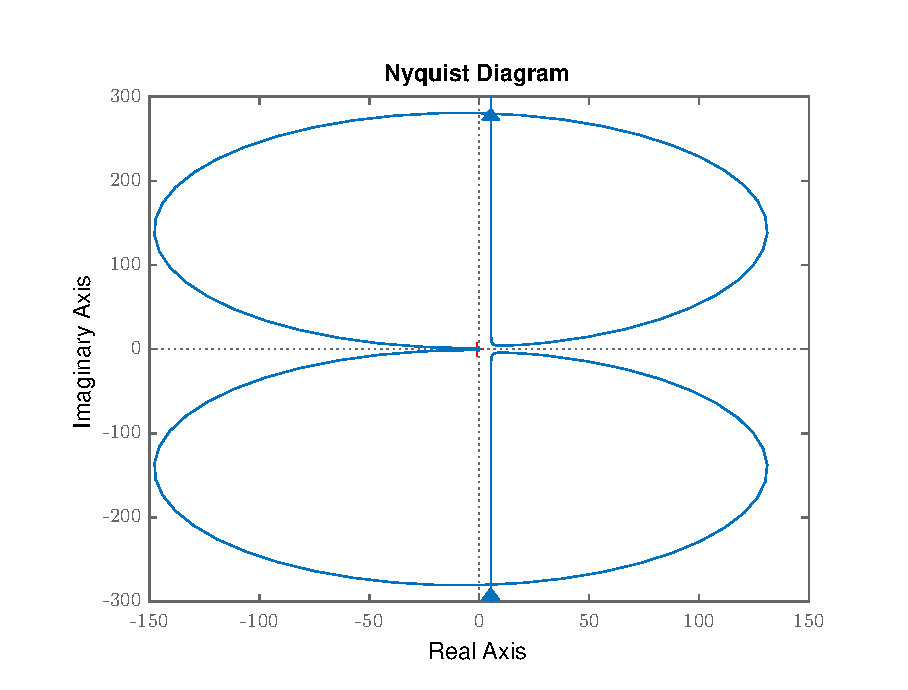
\includegraphics[scale = 0.8]{resources/eps/4-Val/L_nyq.eps}
    \caption{Nyquist plot of the controlled system}
    \label{fig:nyquist-control}
\end{figure}
\begin{figure}[H]
    \centering
    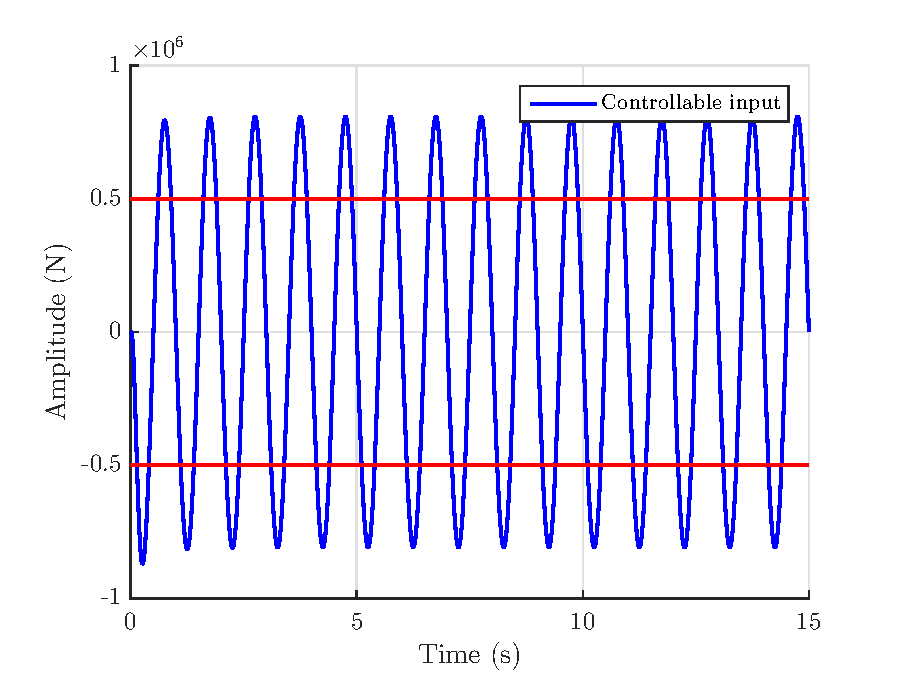
\includegraphics[width=0.8\textwidth]{resources/eps/4-Val/sin_force.eps}
    \caption{Plot of the controllable input of the controlled system subjected to sinusoidal wind}
    \label{fig:controllable-input}
\end{figure}
\begin{figure}[H]
    \centering
    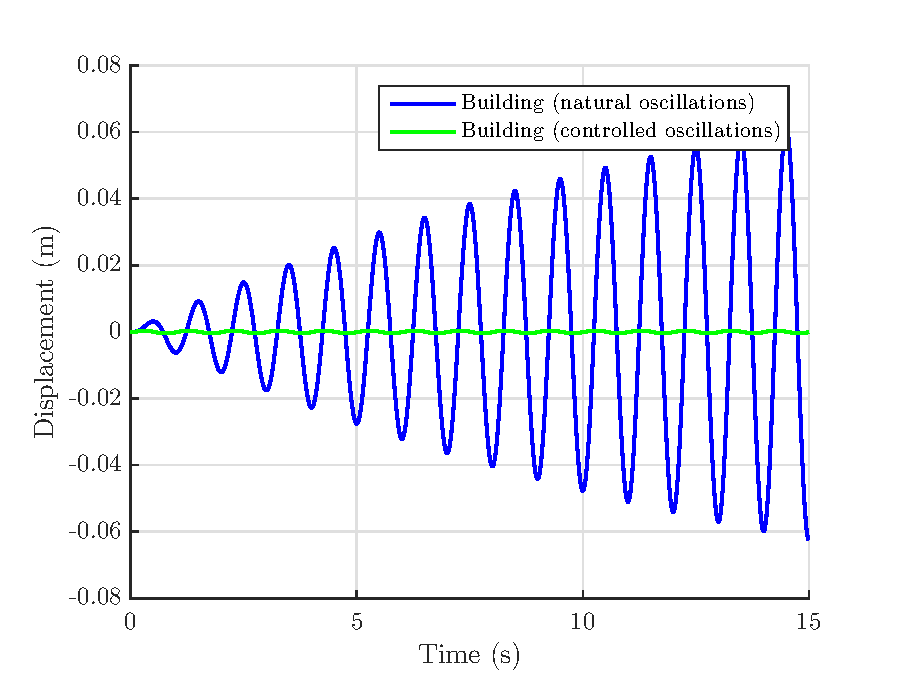
\includegraphics[width=0.8\textwidth]{resources/eps/4-Val/sin_building.eps}
    \caption{Plot of the output of the controlled system subjected to sinusoidal wind}
    \label{fig:output}
\end{figure}
\begin{figure}[H]
    \centering
    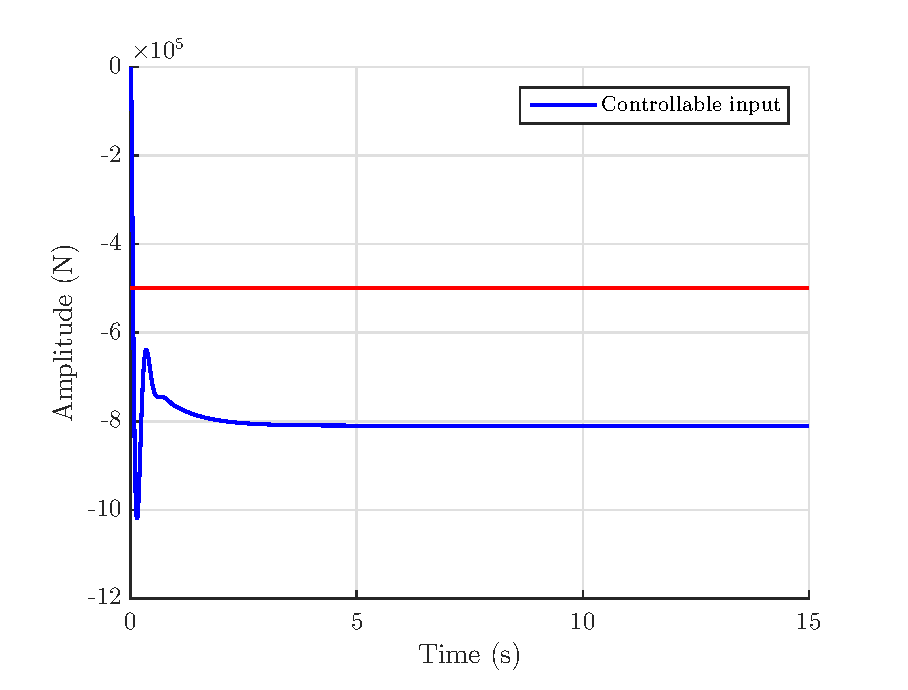
\includegraphics[width=0.8\textwidth]{resources/eps/4-Val/cst_force.eps}
    \caption{Plot of the controllable input of the controlled system subjected to a constant wind}
    \label{fig:controllable-input2}
\end{figure}
\begin{figure}[H]
    \centering
    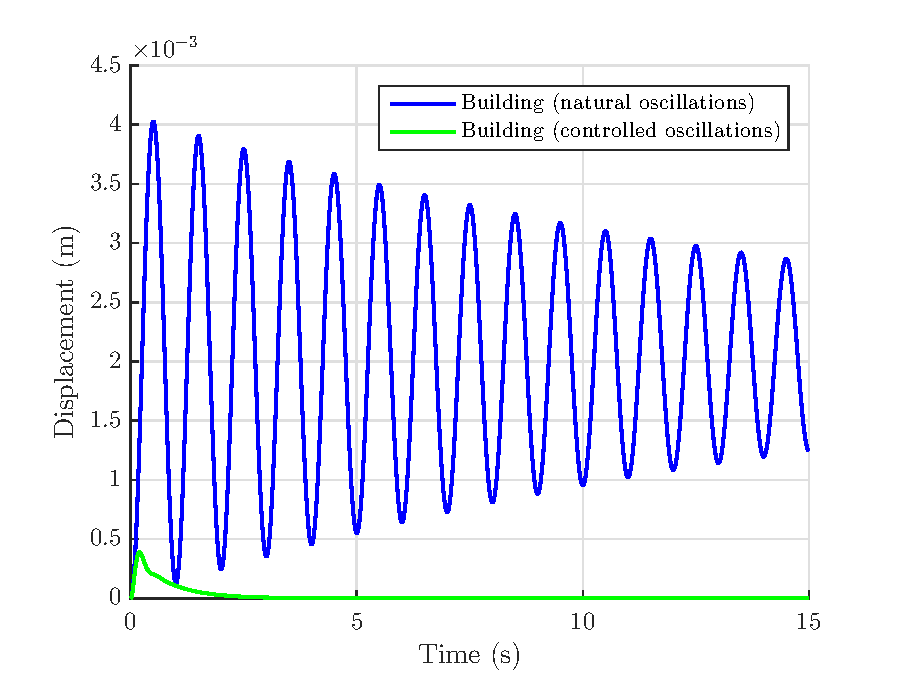
\includegraphics[width=0.8\textwidth]{resources/eps/4-Val/cst_building.eps}
    \caption{Plot of the output of the controlled system subjected to a constant wind}
    \label{fig:output2}
\end{figure}

% Gang of four
\subsection{Gang of four}
\subsubsection{Sensitivity function}
$$
S(s) = \dfrac{1}{1 + PC}
$$
The Bode plots of the sensitivity function are given at figure \ref{fig:sensitivity}. That function tells how the noise acts on the output. We do not want the system to react to the noise, as it is actually the measurement noise that must stay in the output.\par
As noise is a high-frequency phenomenon, we want to have no attenuation of high frequencies in the Bode plot of $S$. As can be seen, it is the case. We have a gain of $0$dB for higher frequencies.\par
In the amplitude graph, we can see a small bump before stabilizing at $0dB$. That is the stability margin, which should remain small. It is not too high in our case, as the maximum sensitivity $M_s = 3.1dB$ and it occurs between $23$ and $24$ rad/s. As the stability margin is equal to the inverse of $M_s$, a high value for $M_s$ would induce a small stability margin and larger amplifications of the disturbances.\newline
\paragraph{Remark}If we wanted a lower gain for lower frequencies (better resistance to disturbance), we would have a greater $M_s$ as, due to Bode's integral formula, the integral of $\log(|S|)$ over $R^+$ is equal to $0$ (waterbed effect). 
\begin{figure}[H]
    \centering
    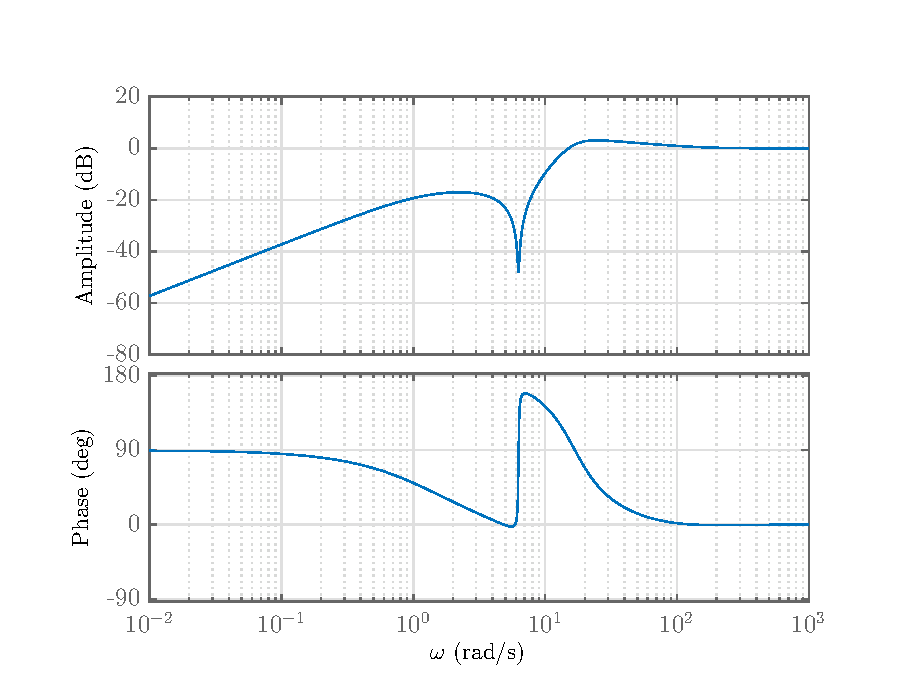
\includegraphics[scale = 0.8]{resources/eps/4-Val/S.eps}
    \caption{Bode plots of the sensitivity function}
    \label{fig:sensitivity}
\end{figure}

\subsubsection{Load sensitivity function}
$$
PS(s) = \dfrac{P}{1 + PC}
$$
This function tells how the disturbances act on the output and the Bode diagrams are given at figure \ref{fig:load}. The system needs to be robust against disturbances. In the present case, these disturbances are low frequency phenomena (frequency of the wind, which we have either chosen constant or a sine function of frequency equal to 1 Hz). We can see that we have a very good reaction concerning the effect of the wind on the output of the system (attenuation of about \SI{-200}{\deci\bel}).
\begin{figure}[H]
    \centering
    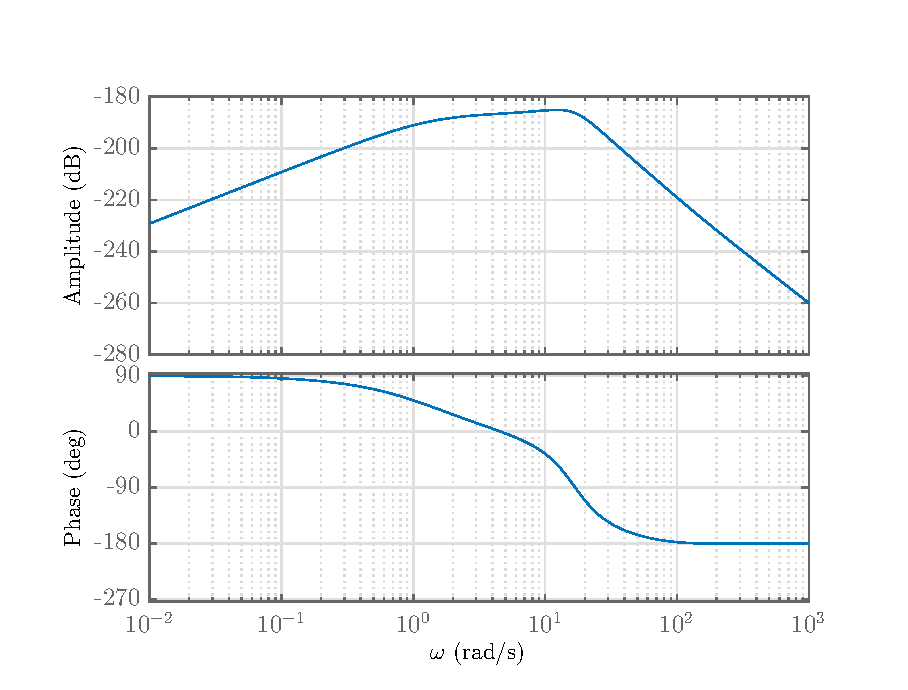
\includegraphics[scale = 0.8]{resources/eps/4-Val/PS.eps}
    \caption{Bode plots of the load sensitivity function}
    \label{fig:load}
\end{figure}

\subsubsection{Complementary sensitivity function}
$$
T(s) = \dfrac{PC}{1 + PC}
$$
This function tells us how the disturbances act on the controllable input and the reference acts on the output and the controllable input, and the Bode diagrams are given at figure \ref{fig:complementary-sensitivity}.\par
The control signal must be reactive to disturbance and the output should be able to track the reference. Amplitudes at low frequency should therefore not be dampened, and one sees that they are not attenuated on the plots. After the maximum complementary sensitivity $M_t$, we have a decreasing slope in amplitude which makes it so that high frequency phenomena (such as noise) are attenuated. (As $S$ + $T$ = 1, we can see that we have a tradeoff between resistance to noise and resistance to disturbance. Better resistance to one induces a worse resistance to the other.)
\begin{figure}[H]
    \centering
    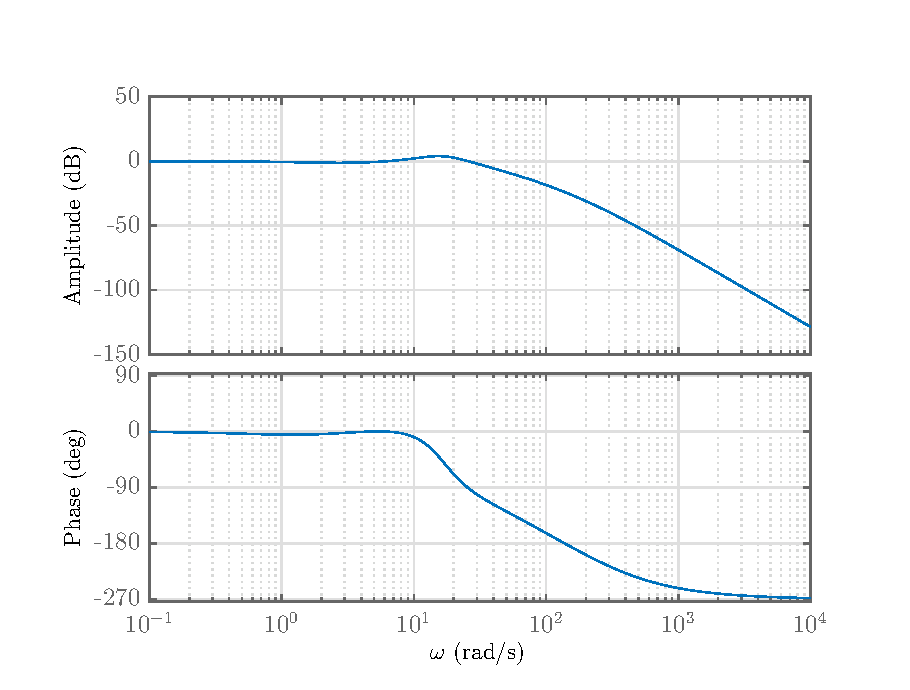
\includegraphics[scale = 0.8]{resources/eps/4-Val/T.eps}
    \caption{Bode plots of the complementary sensitivity function}
    \label{fig:complementary-sensitivity}
\end{figure}

\subsubsection{Noise sensitivity function}
$$
CS(s) = \dfrac{C}{1 + PC}
$$
This function tells us how the noise and the reference act on the controllable input, and the Bode diagrams are given at figure \ref{fig:noise-sensitivity}.\par
That function should be reactive to reference changes, but not to noise, and so have a high magnitude at low frequency and low magnitude at high frequencies. One can see that it is not the case here. Indeed, one has high amplitudes for high frequencies. However, as our reference does not change in our system (we do not plan on dampening the oscillations in a Pisa Tower), it does not really matter.\par
It is also known that temporal domain controllers are better at reacting to reference changes than frequency domain ones.
\begin{figure}[H]
    \centering
    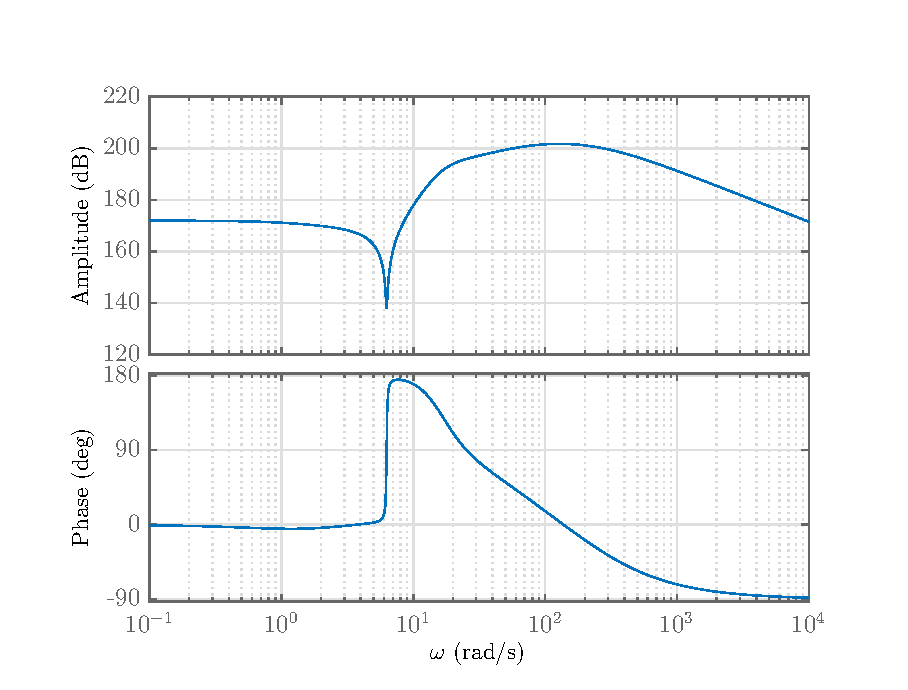
\includegraphics[scale = 0.8]{resources/eps/4-Val/CS.eps}
    \caption{Bode plots of the noise sensitivity function}
    \label{fig:noise-sensitivity}
\end{figure}

% Delays
\subsection{Delays}
The delays in our system are due to the sensor transmitting the information, the microcontroller processing that information and the actuator (piston) actually moving our mass damper. We have chosen that last source of delay as being the biggest one, with a frequency of \SI{50}{\hertz}, which induces delays of \SI{0.02}{\second} (discussed in the lead compensator).\cite{}\par
Some Bode and Nyquist plots showing delays are given at figures \ref{fig:bode-42}, \ref{fig:nyquist-42} and \ref{fig:nyquist-27}. It cannot be seen, but the curve for the delay of $0.02s$ on the Nyquist plot for the lowest phase encompasses the -1 value out of the image.\par
As can be seen, for a phase margin of \SI{42}{\degree}, the delays in our system do not bring instabilities. However, for larger delays, such as the $0.5s$ we have used to simulate Figure \ref{fig:toomuchdelay}, we can clearly see some instabilities in our system. If we wanted to be resistant to such delays, we should increase the phase margin by placing our lag compensator and low-pass filter further away from the crossover frequency.\par
We decided to not include figures comparing the output and the controllable input in the case of delays or not because we ran out of space and we saw almost no difference. The two scenarios reached the same state with only a fraction of a second apart from one another. What happens when the delay is too big, however, is shown in Figure \ref{fig:toomuchdelay}.
\begin{figure}[H]
    \centering
    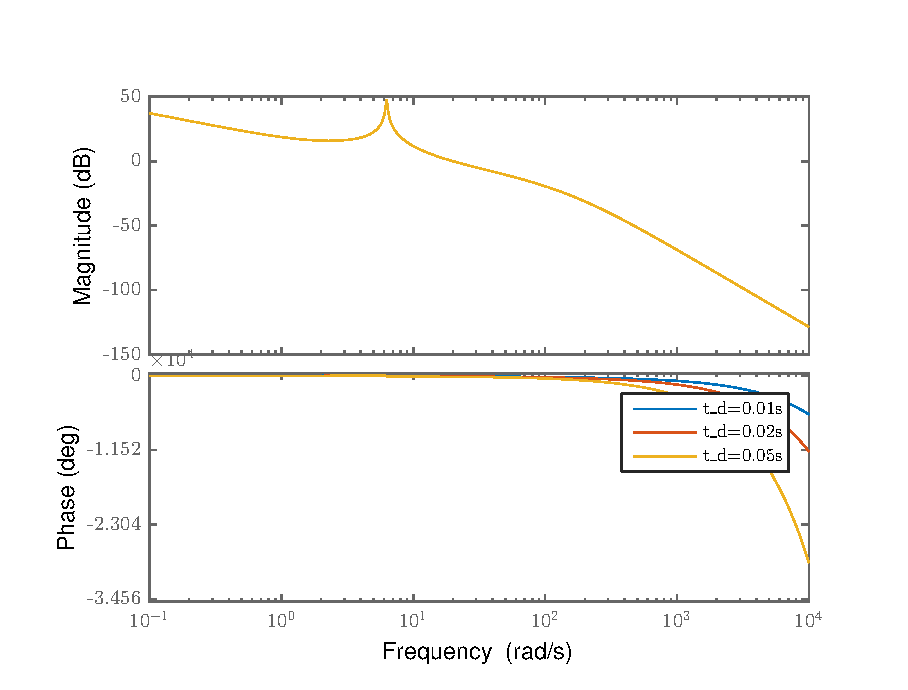
\includegraphics[width=0.8\textwidth]{resources/eps/4-Val/bode_delays.eps}
    \caption{Bode plots for various delays and a phase margin of 42 degrees}
    \label{fig:bode-42}
\end{figure}
\begin{figure}[H]
    \centering
    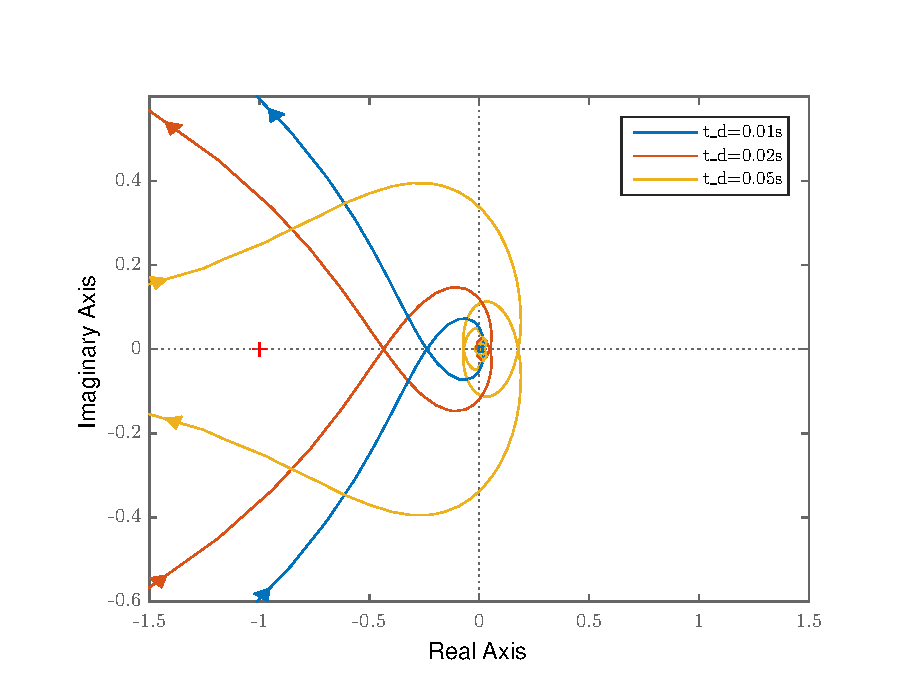
\includegraphics[width=0.8\textwidth]{resources/eps/4-Val/nyq_delay80.eps}
    \caption{Nyquist plots for various delays and a phase margin of 42 degree}
    \label{fig:nyquist-42}
\end{figure}
\begin{figure}[H]
    \centering
    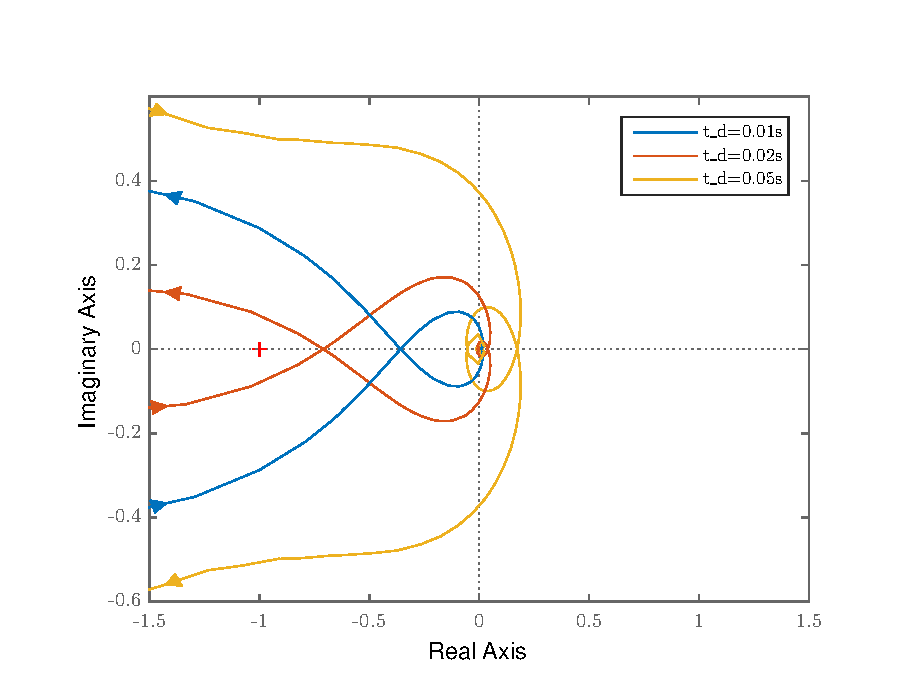
\includegraphics[width=0.8\textwidth]{resources/eps/4-Val/nyq_delay65.eps}
    \caption{Nyquist plots for various delays and a phase margin of 27 degrees}
    \label{fig:nyquist-27}
\end{figure}
\begin{figure}[H]
    \centering
    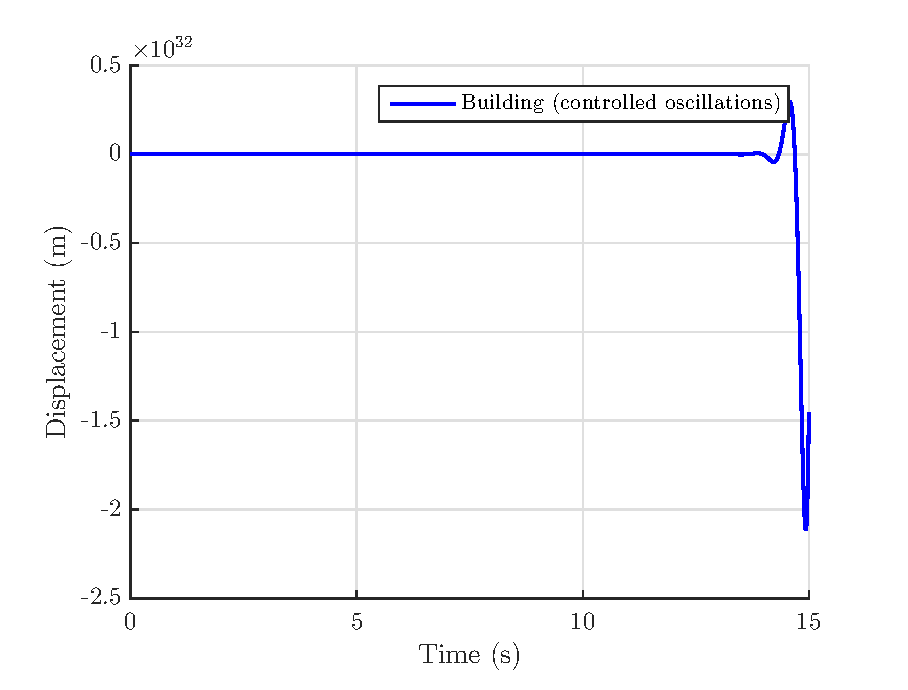
\includegraphics[width=0.8\textwidth]{resources/eps/4-Val/toomuchdelay.eps}
    \caption{Output of our controlled system with a delay of 0.5s}
    \label{fig:toomuchdelay}
\end{figure}

% Noise
\subsection{Noise}
As we can see in Figures \ref{fig:inputnonoise}, \ref{fig:noiselpf} and \ref{fig:noisenolpf}, our system reacts quite well to noise thanks to our low-pass filter. Had we not implemented that filter, we can see that the effect on our controllable input is visible and prone to disturb our control. We did not plot the response of the building as it was not really influenced by noise, whether or not a low-pass filter is added.
\begin{figure}[H]
    \centering
    \includegraphics[scale = 0.7]{resources/eps/input_nonoise.eps}
    \caption{Controllable input of our system with a constant wind and no noise}
    \label{fig:inputnonoise}
\end{figure}
\begin{figure}[H]
    \centering
    \includegraphics[scale = 0.7]{resources/eps/noise_lpf.eps}
    \caption{Controllable input of our system with a constant wind, some noise and a low-pass filter}
    \label{fig:noiselpf}
\end{figure}
\begin{figure}[H]
    \centering
    \includegraphics[scale = 0.7]{resources/eps/noise_nolpf.eps}
    \caption{Controllable input of our system with a constant wind, some noise and no low-pass filter}
    \label{fig:noisenolpf}
\end{figure}

    
    % ----- Conclusion ----- %
    \section{Conclusion}

% Time and frequency domains
\subsection{Time and frequency domains}
The first thing we can observe when comparing the time and frequency controllers is that we do not have a \textbf{static error} in the frequency domain, thanks to the lag compensator. The \textbf{noise rejection} is quite good in both domains. In the time one, it may be explained by the fact that the observer acts as a filter. Indeed, the output of the system being one of the states it has to approximate on the basis of two non noisy inputs and a noisy one, the noise rejection is simplified. For the frequency domain, it is done thanks to the low-pass filter.\par
Concerning the reaction to a \textbf{reference change}, we found out that the frequency controller allowed us to reach that reference before $3s$, at the cost of an unbelievably high force applied on the damper. It is not plotted because we ran out of space and it was not asked explicitly, but we have a spike at $1.3m$ for the displacement of the building then a stabilization at 1m. It is not the case for the time domain, where we have huge displacements and no stabilization that we can observe in a reasonable time. That is counter-intuitive as we thought that a controller in time domain would track a reference better than one in frequency domain.\par
Concerning the \textbf{delays}, the frequency domain deals with them more easily than the time domain, although not by much. Indeed, as can be seen in Figure \ref{fig:delay}, the time controller is also quite good with small delays ($0.02s$).
\begin{figure}[H]
    \centering
    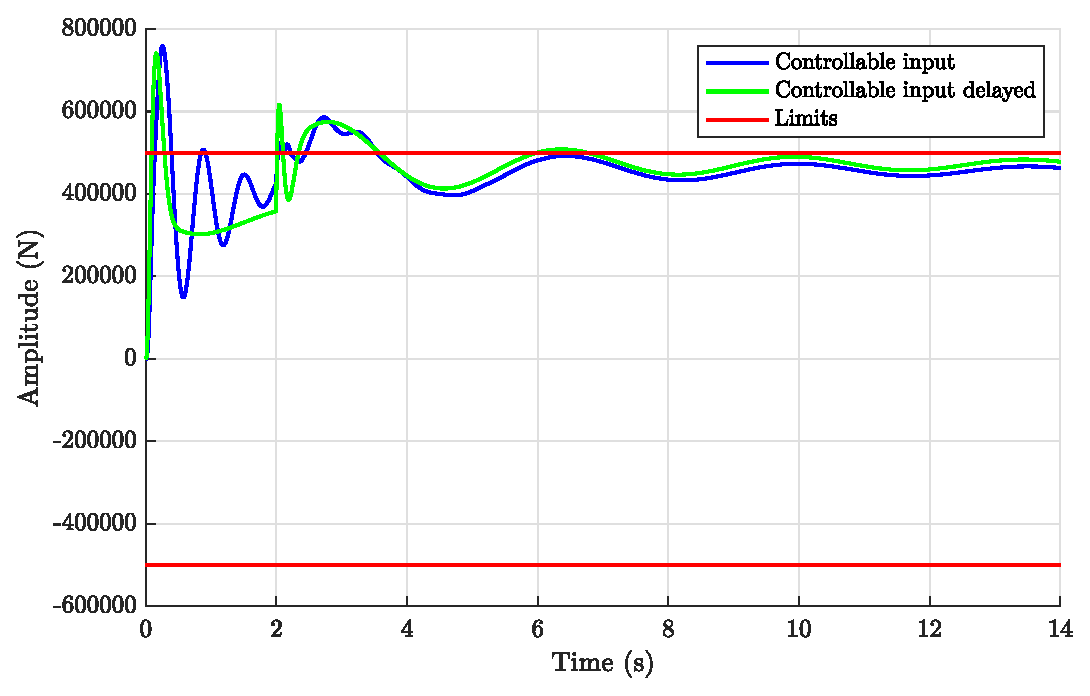
\includegraphics[scale = 0.7]{resources/eps/3_delay-controllable-input.eps}
    \caption{Time controller simulation with 0.02s of delay.}
    \label{fig:delay}
\end{figure}

% General conclusion
\subsection{General conclusion}
This project allowed us to put in practice a lot of concepts that were explained in the theoretical lectures. However, we could not reach controllers that complied with the constraints Pr Denoël gave us (an acceleration between $0.3$ and $0.6g$). This may come from the fact that some parameters had wrong values or that we oversimplified the problem.\par
We played with the different parameters of our controllers a huge amount of time in order to reach these constraints and the results presented in this report are the best we could manage. Using a bigger mass for the damper would have helped us reach our constraints, but we felt like $30$ tons was already very heavy. We have thus decided to use an acceleration that was high, but not completely out of touch with reality. Although our results are not perfectly aligned with our initial constraint, we feel like we have understood the theoretical concepts we have applied, which was ultimately the goal of this project.

    
    % ----- References ----- %
    \newpage
    \subsection{References}
    \nocite{*}
    \printbibliography
\end{document}
